%%
%%
\documentclass[preprint,3p,10pt,onecolumn,number,sort&compress]{elsarticle}
%\documentclass[final,3p,10pt,twocolumn,number,sort&compress]{elsarticle}



%% if you use PostScript figures in your article
%% use the graphics package for simple commands
%% \usepackage{graphics}
%% or use the graphicx package for more complicated commands
 \usepackage{graphicx}
 \usepackage{amsmath}
 \usepackage{stfloats}
 \usepackage{afterpage}
 \usepackage{placeins}
% \usepackage{xfrac}

%% or use the epsfig package if you prefer to use the old commands
%% \usepackage{epsfig}

%% The amssymb package provides various useful mathematical symbols
\usepackage{amssymb}
\usepackage{color}
%% The amsthm package provides extended theorem environments
%% \usepackage{amsthm}

%% The lineno packages adds line numbers. Start line numbering with
%% \begin{linenumbers}, end it with \end{linenumbers}. Or switch it on
%% for the whole article with \linenumbers after \end{frontmatter}.
%% \usepackage{lineno}




%\journal{Journal of Nuclear Materials}
\usepackage{lipsum}
\makeatletter
\def\ps@pprintTitle{%
 \let\@oddhead\@empty
 \let\@evenhead\@empty
 \def\@oddfoot{}%
 \let\@evenfoot\@oddfoot}
\makeatother
\begin{document}

\begin{frontmatter}


\title{\textit{Ab initio} molecular dynamics (AIMD) simulations of NaCl, UCl$_3$ and NaCl-UCl$_3$ molten salts}

\author[label1]{D. A. Andersson}
\ead{andersson@lanl.gov}
\author[label2,label3]{B. W. Beeler}
\address[label1]{Los Alamos National Laboratory}
\address[label2]{North Carolina State University}
\address[label3]{Idaho National Laboratory}


\begin{abstract}
\textit{Ab initio} molecular dynamics (AIMD) simulations are used to calculate select thermophysical %(density, thermal expansion, compressibility and diffusivity) 
and thermodynamic %(mixing energy and heat capacity) 
properties of NaCl, UCl$_3$ and NaCl-UCl$_3$ molten salts. Following established approaches, the AIMD simulations %use either the PBE or XX exchange-correlation potentials and 
include a model for Van der Waals interactions. The Langreth \& Lundqvist, DFT-D3 and dDsC dispersion models are first tested for molten NaCl in order assess their accuracy for density and heat capacity predictions across a range of temperatures. %Either constant pressure or constant volume ensembles were used for the simulations. 
%All methods predict densities within 10\% of the experimental data, with the dDsC and Langreth \& Lundqvist methods being within 5\%. 
Based on the NaCl results, the Langreth \& Lundqvist and dDsC methods are extended to the UCl$_3$ system and compared to available experimental data. %The dDsC dispersion model exhibits slightly better agreement with experiments for both density and heat capacity, as compared to the NaCl system.  
%which is followed by mixtures of UCl$_3$-NaCl. Accurate results 
 % with a few select simulations performed for the DFT-D3 model. %The Langreth \& Lundqvist methodology... 
%The dDsC method predicts densities within a few per cent of the experimental data for UCl$_3$. The Hubbard $U$  model increases the volume for all cases and results in slightly lower density than for the case where it is not included. 
Next, mixtures of NaCl-UCl$_3$ are investigated and analyzed with respect to the deviation from ideal solution behavior. % for a wide range of temperatures. 
For the dDsC simulations, density deviates by up to 2\% from an ideal mixture, with the maximum occurring close to the eutectic composition, %(about 30\% UCl$_3$), 
possibly shifted slightly towards the NaCl rich side. The temperature dependence of the deviation from ideal solution is weak in the NaCl rich region, but more discernible in the UCl$_3$ rich region. %, which results in a non-ideal behavior of the temperature dependence of density in this region. %The Langreth \& Lundqvist simulations do not predict a systematic deviation from an ideal solution. 
The mixing energy also deviates from an ideal solution and exhibits a minimum of about -0.07 eV per formula unit, again close to the eutectic composition, but this time shifted slightly towards the UCl$_3$ rich region. Within the uncertainty of the simulations, the mixing energy does not depend on temperature. %, which results in heat capacity behaving according to an ideal solution.  
The trends observed for mixing properties are rationalized by correlating them to the coordination chemistry, which emphasizes the competition between increasing the Cl coordination around U ions and maintaining the extended network formed by U and Cl ions as the NaCl concentration increases. The density and mixing energy predictions are also compared to existing experimental measurements. %Finally, the constant volume simulations allow determination of the compressibility and diffusivity, which are presented for select cases. The simulation results are compared to available experimental data.
\end{abstract}

%\begin{keyword}
%% keywords here, in the form: keyword \sep keyword

%% MSC codes here, in the form: \MSC code \sep code
%% or \MSC[2008] code \sep code (2000 is the default)

%\end{keyword}

\end{frontmatter}

%%
%% Start line numbering here if you want
%%
% \linenumbers

%% main text
\section{Introduction}
\label{sec:intro}
Molten salt reactors (MSRs) are among the advanced concepts pursued under the generation IV nuclear energy technology umbrella. However, the basic concept is not new and was first developed as part of the effort to power aircrafts with nuclear energy in the 1950's. Later in the 1960's, Oak Ridge National Laboratory (ORNL) built and operated the Molten-Salt Reactor Experiment (MSRE)~\cite{MSRE}. This reactor used a fluoride salt with uranium as fuel. Fluoride salts are still highly relevant and proposed in several designs. In addition, chloride salts are being considered for MSRs operating in the fast neutron spectrum. The present study focuses on chloride salts, in particular the NaCl-UCl$_3$ system, which is one of the primary fuel salt candidates.

%Property data for chloride salts are in many cases limited and sometimes of unknown accuracy. This is especially true as actinides (U, Pu), impurities, and corrosion and fission products are added. Using atomic scale simulations to fill these data gaps and to provide mechanistic understanding of property relations would facilitate more accurate evaluation of various concepts by reactor designers, developers and other interested parties. Modeling and simulations have an important role to play in reducing data gaps, because the compositional space of interest is extensive and difficult to cover with experiments alone, especially since some of the salts are also highly toxic and radioactive. This benefit is already acknowledged  in the literature~\cite{Li,Li2020,Nam2014,Nam2015,SONG}, but the field is still evolving and many properties are either only partially explored or remains to be investigated, in particular for complex compositions. 

Experimental characterization of UCl$_3$ densities have been reported by Janz et al.~\cite{Janz1988} and Desyatnik et al.~\cite{Desyatnik}. The density correlations derived from these two experimental data sets deviate significantly from each other. Desyatnik et al.~\cite{Desyatnik} also investigated the density of NaCl-UCl$_3$ mixtures. They identified a negative deviation from an ideal solution across most of the composition range, with the high-temperature UCl$_3$ rich region deviating slightly from this trend. 
Maatsura et al.~\cite{Matsuura} measured the mixing energies of NaCl-UCl$_3$ at 1173 K, which highlighted a negative deviation from ideal solution behavior (exothermic reaction) with a  minimum of $-0.07$ to $-0.08$ eV per formula unit close to the eutectic composition ($x\approx 0.35$, where $x$ is the UCl$_3$ fraction), but perhaps slightly shifted towards the 50-50 composition. There are two Calphad assessments of the NaCl-UCl$_3$ system~\cite{BENES2008, YIN2020}. The magnitude and shape of the NaCl-UCl$_3$ mixing energies are noticeably different between the two assessments~\cite{YIN2020}. The assessment by Benes et al.~\cite{BENES2008} arrived at a form with a minimum close to the eutectic composition, while Yin et al.~\cite{YIN2020} used the experimental data due to Matsuura et al.~\cite{Matsuura} as input, which resulted in a more negative mixing energy that is shifted slightly closer to the 50-50 composition. The magnitude of the mixing energy is off by about 50\% between the two assessments. 

The sparse and sometimes contradictory experimental data on molten salts in general, and the NaCl-UCl$_3$ system in particular, provides justification for pursuing modeling and simulations as a complementary approach to gain improved understanding. This opportunity is already acknowledged  in the literature. Both classical molecular dynamics (CMD) and \textit{ab initio} molecular dynamics (AIMD) simulations have been used to study chloride salts involving actinides~\cite{Li,Li2020,Nam2015,SONG}. Li et al.~\cite{Li} used AIMD simulations to study the local structure of UCl$_3$, UCl$_4$, and mixtures of UCl$_3$, UCl$_4$ and NaCl at 1173 K. This study showed good agreement with experiments for the radial distribution function of the first coordination shell and identified network formation of UCl$_3$ units in mixed NaCl-UCl$_3$ salts~\cite{Li}. %radial distribution function. 
In order to study temperature dependent thermo-physical properties, a semi-empirical potential was developed~\cite{Li2020}. This potential successfully predicted density, thermal conductivity, and viscosity, though validation is challenged by the lack of experimental data. Nam et al.~\cite{Nam2015} studied the solution thermodynamics of dilute concentrations of UCl$_3$ in a base salt and investigated the properties of base salts for different Van der Waals interaction models. Song et al.~\cite{SONG} performed AIMD simulations of densities and transport properties in a LiCl-KCl eutectic salt with a small concentration of UCl$_3$. 

In the present study, AIMD simulations relying on different models for the Van der Waals interactions were used to predict temperature dependent thermophysical (density) and thermochemical (mixing energy and heat capacity) properties of NaCl, UCl$_3$ and NaCl-UCl$_3$. The standard PBE exchange-correlation potentials typically used were extended to include a Hubbard $U$ model for the actinide 5f electrons. This extension has not previously been utilized for studying actinide salts. The purpose of the study was first to determine with what accuracy fundamental properties can be predicted with AIMD simulations for actinide containing salts, second to populate some of the data gaps that exist in the literature, and third to provide understanding of the link between coordination chemistry and properties. 

This paper is organized as follows. The methodology is described in Sec. \ref{sec:method}, followed by results and discussion in Sec. \ref{sec:results}. First, the benchmark for NaCl is presented, after which the UCl$_3$ results are reviewed followed by NaCl-UCl$_3$ mixtures. The implications of our results are discussed in Sec. \ref{sec:discussion} and, finally, our conclusions are presented in Sec. \ref{sec:conclusions}. 

\section{Methodology}
\label{sec:method}
The AIMD simulations were performed with the VASP code~\cite{Kresse1996}. All simulations used the $\Gamma$ point for integration in reciprocal space. The accurate simulation setting was utilized in VASP, but the plane wave cut-off energy was increased above the standard setting to 400 eV. Gaussian smearing with a smearing parameter of 0.05 eV was used for the partial occupancies of the wave functions. The convergence criteria for the electronic minimization was at least 10$^{-3}$ eV for NaCl and $5\times10^{-3}$ eV for salts containing uranium. The Projector Augmented Wave (PAW) method was used to describe the core electrons~\cite{PAW1,PAW2}. The PAW potentials supplied with VASP for the PBE exchange-correlation potential were utilized, unless otherwise noted. For Na, both the pseudopotential version that only includes the \textit{s} electron(s) in the valence shell and the version that also includes the semi-core \textit{p} electrons were utilized. The difference between the two potentials will be discussed in Sec. \ref{sec:results}. The PAW potential for Cl also included \textit{p} electrons and for U it included the outer \textit{s}, \textit{p}, and \textit{f} electrons in the valance shell. 

\subsection{Supercell Size}
The simulations used a range of supercell sizes with the largest consisting of 216 (NaCl), 216 (UCl$_3$) and 134-184 (NaCl-UCl$_3$ mixtures) atoms. The smallest cells for the same systems contain 64, 64 and 60-72 atoms, respectively. Further details will be provided in Sec. \ref{sec:results}. 
For NaCl and UCl$_3$ the supercells were created by one of two methods. In the first method, the crystalline unit cell is replicated to generate a supercell, followed by melting of the lattice by performing high temperature MD simulations. The mixed supercells were created by replacing Na ions with U ions or vice versa, in some cases additional molecular units were added to ensure that a suitable number of atoms were maintained in the supercells. In the second method, the PACKMOL package \cite{packmol} was utilized to randomly insert individual molecules of NaCl and UCl$_3$ in the targeted concentration, followed by high temperature equilibration. 

The differently sized supercells were investigated in order to understand and optimize the compromise between computational efficiency, enabling sampling in the time domain, and accuracy with respect to long range interactions. The radial distribution function (RDF) was used as the most basic measure of the adequacy of the supercell size, with convergence with respect to the targeted thermophysical and thermodynamic properties following suit. All the supercells investigated properly capture the expected radial distribution function in the liquid state. This behavior is exemplified in Figures \ref{fig:radial}a) and \ref{fig:radial}b) for UCl$_3$ and NaCl supercells of different size, respectively. The smaller cells predict essentially identical radial distribution functions as compared to the larger cells, but enable improved computational efficiency. Although the larger cells may still be more accurate for, e.g., mixed salts exhibiting more complex radial distribution functions, the situation in mixed salts is further complicated by the need to sample sufficient configurations to resolve the preferred short and intermediate range distribution of ionic species in network forming salts such as UCl$_3$~\cite{Li}, which requires fairly long simulation times. Proper sampling is easier to achieve in smaller supercells given the computational cost of AIMD simulations, even though the radial distribution itself, as well as other properties, may be better described in a larger supercell. For this reason, the results in Sec. \ref{sec:results} tend to use supercells of intermediate size.  Based on the verification against large supercells for the radial distribution function above and further examples in Sec. \ref{sec:results}, the results in the present study are considered sufficiently converged with respect to supercell size.

\begin{figure*}[htb]
\centering
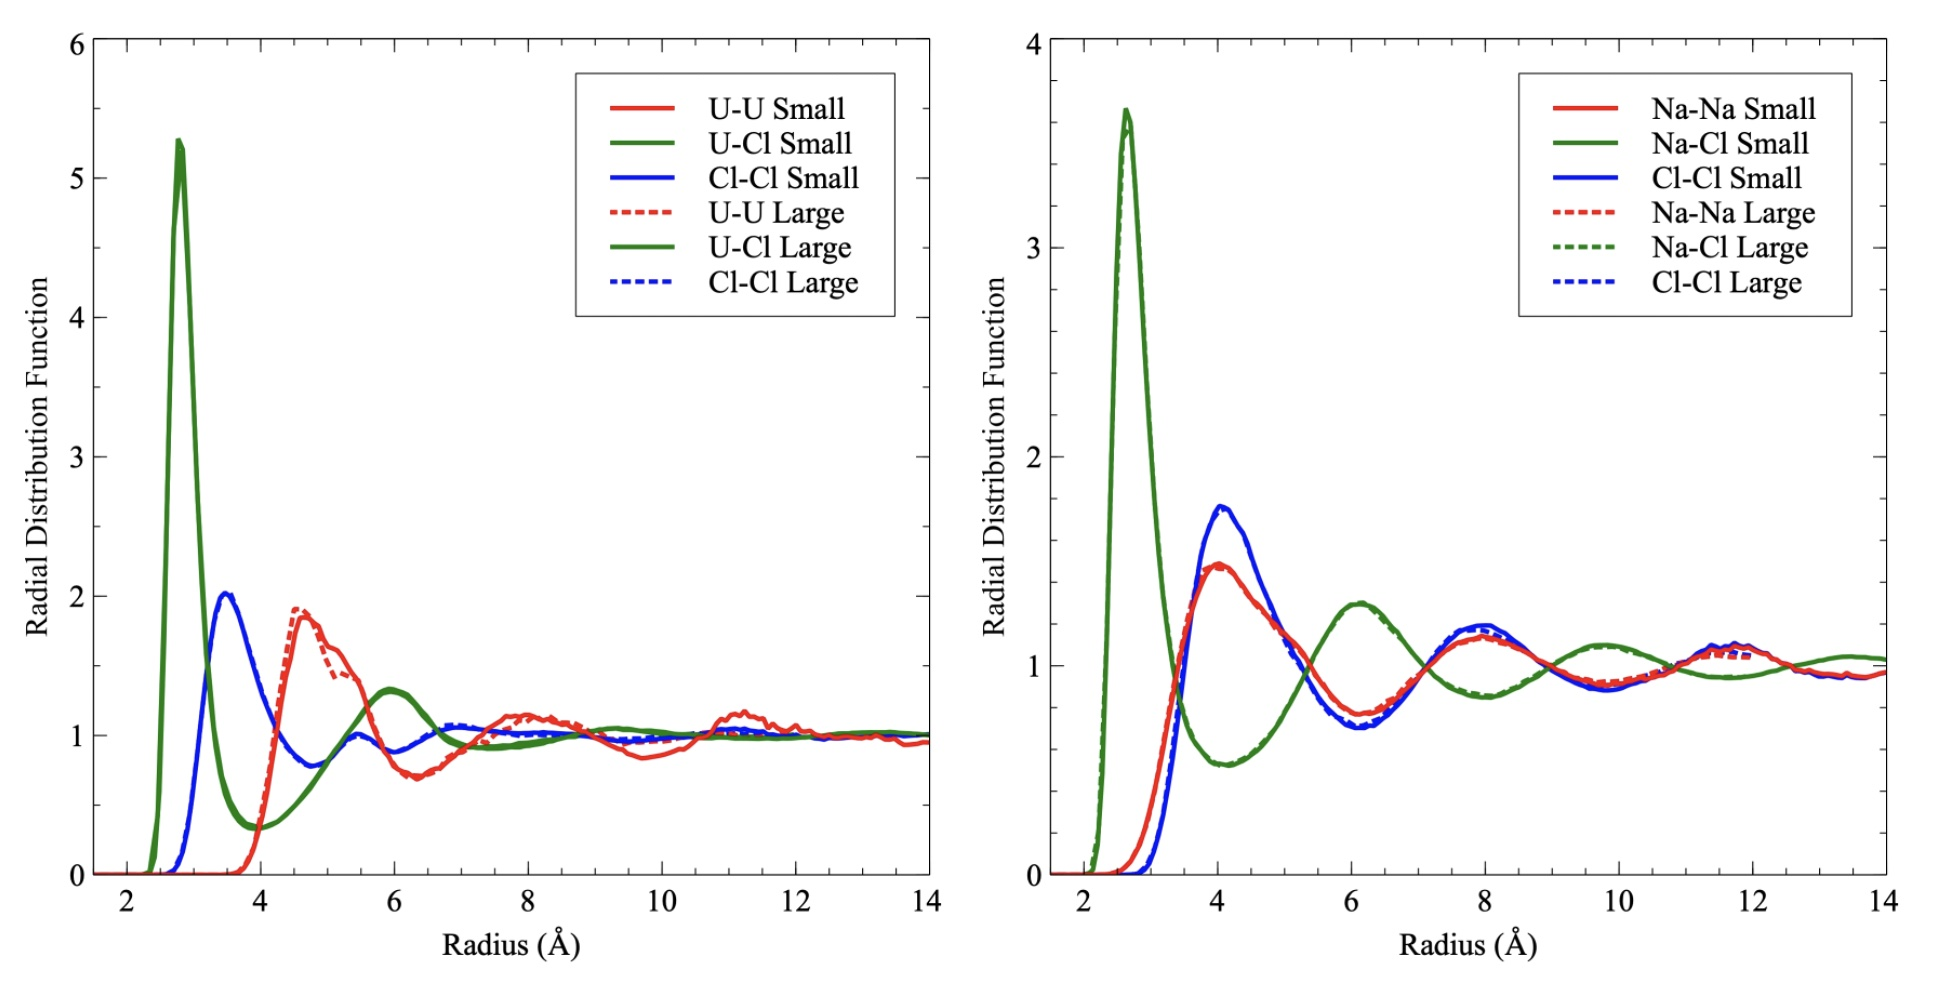
\includegraphics[width=0.9\textwidth]{fig1.jpg}
\caption{The predicted radial distribution function in a) UCl$_3$ and b) NaCl obtained by supercells containing 64 (small) and 216 (large) atoms at 1250 K.} 
\label{fig:radial}
\end{figure*}

%\FloatBarrier

\subsection{Application of the Hubbard U term}

The generalized gradient approximation can fail to describe systems with localized (strongly correlated) \textit{f} electrons. This is often remedied by applying a Hubbard-like term to treat the strong on-site Coulomb interaction, commonly referred to as DFT+U (also LDA+U or GGA+U) \cite{rohrbach2003}. Determination of the appropriate magnitude of the applied screening needs to be uniquely determined for each element within each compound. The rotationally invariant approach of Dudarev \cite{dudarev1998} was implemented to investigate the effects of Coulombic screening, with the vdW-DF2 Van der Waals functional. The density, bandgap, and energy per molecule were analyzed as a function of U-J (U$_{eff}$) in increments of 1 eV for both UCl$_3$ and NaCl-33UCl$_3$ at 1250 K, in the ferromagnetic (FM) and anti-ferromagnetic (AFM) states. It should be emphasized that the Hubbard U term was only applied  the \textit{f} electrons of uranium. 

The zero-pressure density was determined by constructing pressure as a function of volume curves as a function of U$_{eff}$ at 1250 K for both the FM and AFM states. As will be discussed later, there is not an exact correspondence between the AIMD predicted densities and the experimental densities, but reasonable agreement is achieved. There exists a general trend of decreasing density with increasing U$_{eff}$, and that the AFM state predicts a slightly higher density (lower volume) than the FM state. These zero-pressure volumes are then utilized to determine the electronic density of states and the energy per molecule of their respective systems. A full discussion of densities is included in Sec. \ref{sec:results}. 

The electronic density of states of AFM UCl$_3$ with a U$_{eff}$ of 0 and 4 eV is shown in Fig. \ref{fig:DOS}a. It can be seen that at a U$_{eff}$ of 0 eV with no Coulombic screening, UCl$_3$ exists electronically as a conductor. It is known that this molten salt exhibits insulating properties {\color{red}(need citation)} with at least a minimal band gap. With the application of the Hubbard U term, an insulating electronic structure is induced, as can be seen in Fig. \ref{fig:DOS}b. The magnitude of the bandgap changes as a function of the magnitude of U$_{eff}$, with no bandgap below 2 eV, and the bandgap progressively increasing up to approximately 2.3 eV for a Ueff of 5 eV. The magnitude of the bandgap of UCl$_3$ has not been experimentally determined, removing the possibility of fitting the U$_{eff}$ to the experimental bandgap. 

It was also observed that the preferred magnetic state changes as a function of U$_{eff}$, with FM being preferred in the low U$_{eff}$/conducting region, and the AFM state preferred in the high U$_{eff}$/insulating region. This was identified by analyzing the energy per formula unit as a function of Hubbard U magnitude. It is presumed that at high temperatures there would not be an ordered series of spins, and that is confirmed within this work, given that the electronic structure is appropriately accounted for. A previous study \cite{Li} investigated UCl$_3$ in the FM state without DFT+U corrections. Although it was shown above that this incorrectly produces an electronically conductive molecular system, the choice of the FM state, given the absence of a Hubbard U term, is not wholly incorrect. For a U$_{eff}$ value of 0, the FM state is the energetically preferred form of magnetism.  

It is clear that a value of U$_{eff}$ greater than 2 eV is required to ensure the proper insulating electronic structure, and that this system prefers an AFM state. However, the actual magnitude of the optimal U$_{eff}$value remains unclear. Thus, a further analysis on NaCl-33UCl$_3$ was performed to observe what trends in the electronic structure and energy per molecule exist as a function of U$_{eff}$. It was observed that at a U$_{eff}$ value of greater than 1 eV, an insulating electronic structure was induced, while the absence of the Hubbard U term yielded a conducting system. Additionally, the AFM state becomes energetically favorable above a U$_{eff}$ of 2 eV. The trends in the density for NaCl-33UCl$_3$ as a function of U$_{eff}$ are statistically indistinguishable from those for UCl$_3$. This investigation served to reinforce the findings that value of U$_{eff}$ greater than 2 eV is required to ensure the proper insulating electronic structure, and that the NaCl-UCl$_3$ system prefers an AFM state. 

Finally, the constrained DFT linear-response method \cite{PhysRevB.71.035105} was utilized within the Lichtenstein approach \cite{PhysRevB.52.R5467} for the Hubbard U term of UCl$_3$. An approximate U value range of 3.0-4.5 eV was determined and the J value was set to 0.51 eV. These values are similar to those proposed for UO$_2$ \cite{dudarev}. Given the lack of high-fidelity experimental data to serve as a basis for optimization of the Hubbard U magnitude, it was determined that a U$_{eff}$ value of 4 eV (in the case of Dudarev) or a U value of 4.5 eV and a J value of 0.51 eV (in the case of Lichtenstein) should be utilized for the NaCl-UCl$_3$ system. Differences between the two implementations of the Hubbard U term should be statistically insignificant.

\begin{figure*}[h]
\centering
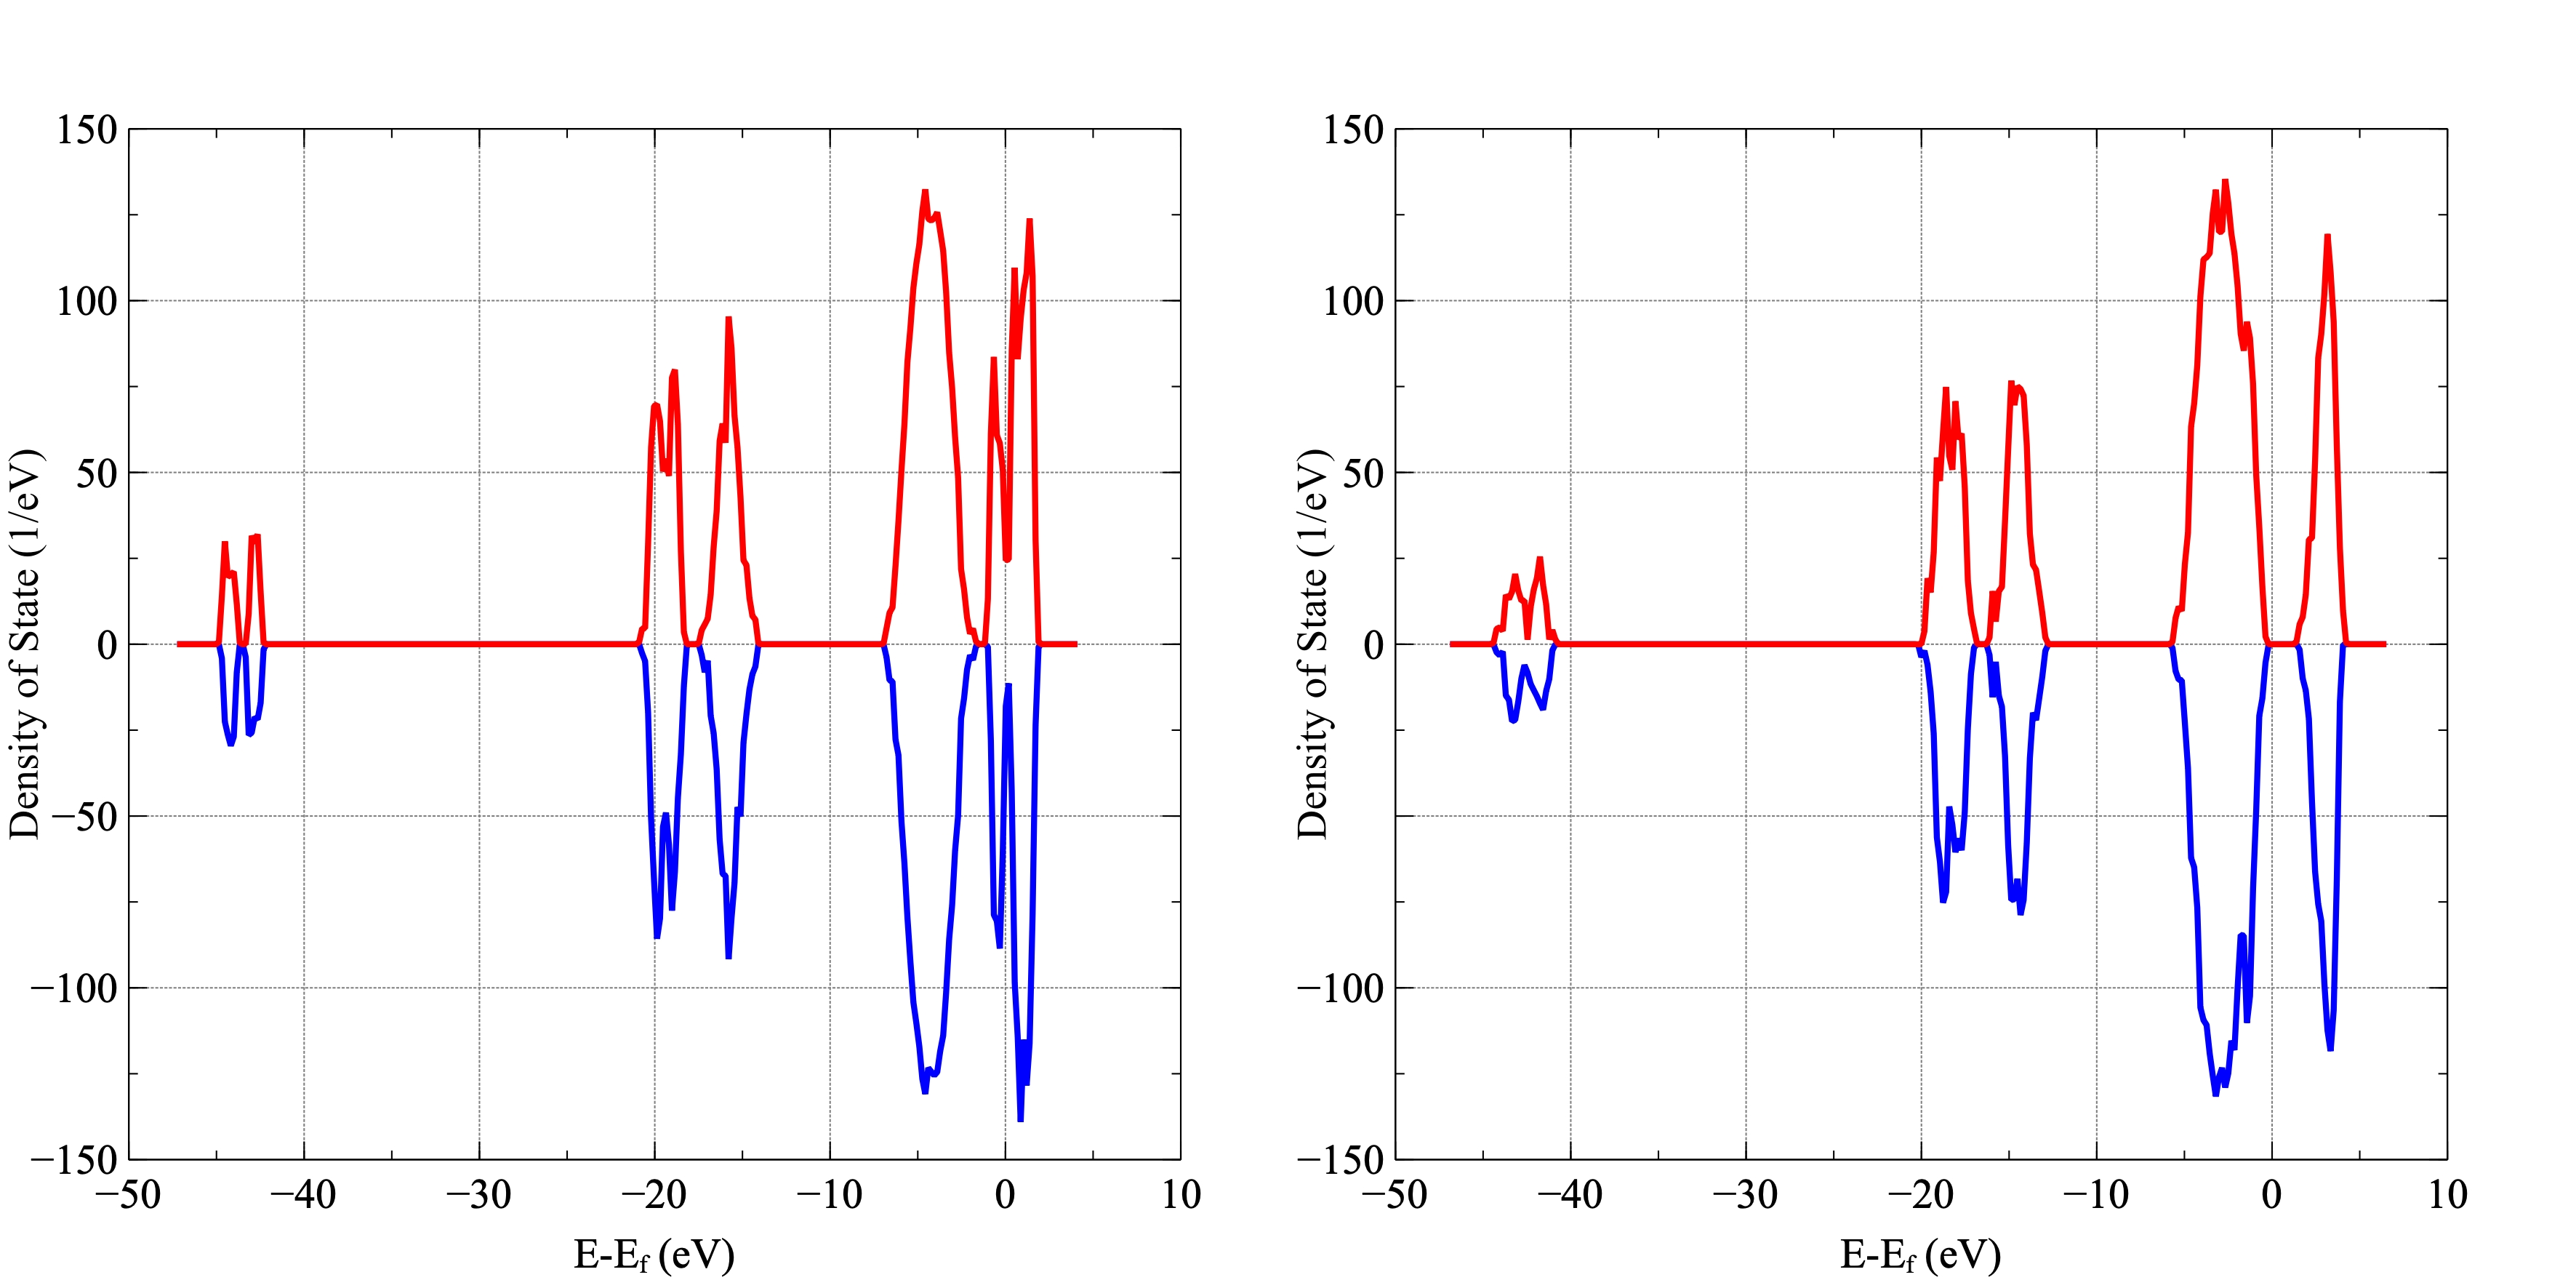
\includegraphics[width=0.9\textwidth]{fig2.jpg}
\caption{The predicted density of states for simulations of molten UCl$_3$ at 1250 K, a) including (AFM) and b) not including (FM) a Hubbard $U$ model. {\color{red} Furhter details to be added.}} 
\label{fig:DOS}
\end{figure*}

%\FloatBarrier

\subsection{Van der Waals Dispersion}

It is well-established in the literature that Van der Waals or dispersion interactions are critical for reproducing the density of molten salts by DFT methods~\cite{Li,Nam2014,Nam2015}. In general, density functional theory methods are unable to describe van der Waal dispersion (vdW) forces. A pragmatic method to work around this problem is to add a correction to the conventional Kohn-Sham DFT energy. This is performed through the addition of a vdW correction, or a replacement of the exchange-correlation functional to account for dispersion interactions. Given that there are numerous implementations of dispersion interaction, the choice of which dispersion interaction to utilize can be material and system dependent, and unknown without prior testing. Previous simulations have used both the DFT-D3~\cite{Li,Grimme} and the Langreth \& Lundqvist~\cite{Nam2015,Dion,Klimes} (vdW-DF2) methodologies for various molten chloride salts. Both methods were used in the present study. In addition, the density-dependent energy correction (dDsC) method~\cite{Steinmann2011,Steinmann2} was used with the goal of improving accuracy. The dDsC method does not include parameters for \textit{f} elements in the standard VASP version. In order to enable simulations the corresponding parameters were taken from Ref. ~\cite{Kim}. 

\subsection{AIMD simulations}
The AIMD simulations for the molten salt supercells were performed using isobaric (NPT) conditions. The primary intent of the NPT simulations (with the pressure set to zero) is to evaluate density, thermal expansion, heat capacity and mixing energy. All NPT ensemble simulations used the the Langevin thermostat in VASP. For the NPT simulations, the temperature friction coefficient was set to 10 ps$^{-1}$ and the friction coefficient for the lattice degrees of freedom to 1 ps$^{-1}$. The time step was set to 2 fs for production runs between \~1000 K and 1500 K. Around and below 1000 K a larger time step, up to 5 fs, is warranted due to the slow dynamics of uranium ions.

The simulations used pre-equilibrium and equilibration runs that involve melting the lattice and ensuring convergence of the total energy and pair distribution function for the temperature of interest. After pre-equilibration and equilibration, production runs follow for at least 20 ps. Some simulations used longer production runs, in particular this applies to the simulations based on smaller supercells (up to 50 ps) and systems containing a mixture of UCl$_3$ and NaCl (up to 40 ps). NPT simulations require long equilibration runs and may sometimes leave the equilibrium state due to distortions of the supercells, which is in part a consequence of applying the technique to somewhat small supercells. All simulations were inspected to avoid sampling such regimes. Additionally, an NVT ensemble was applied to obtain compressibilities, densities, heat capacities, and diffusivities. Only the vdW-DF2 dispersion functional was utilized for NVT ensembles. 

Properties were calculated by averaging over the production run (not including the equilibration or pre-production time). Densities were trivially obtained from the supercell volume and heat capacities from the slope of the total internal energy ($E_{tot}$) as function of temperature. 
\begin{equation}
\label{eq:cp}
C=\frac{\partial E_{tot}}{\partial T}
\end{equation}
For the NPT ensemble, this corresponds to heat capacity at constant pressure ($C_p$), and for the NVT ensemble heat capacity at constant volume (C$_V$). Mixing energies were calculated from the potential energy ($E_{pot}$) of the mixed salt with pure NaCl and UCl$_3$ at the same temperature as the reference. 
\begin{equation}
\begin{split}
E_{mix}=E_{pot}(U_xNa_yCl_{3x+y})-xE_{pot}(UCl_3)-yE_{pot}(NaCl)
\end{split}
\end{equation}

The compressibility is calculated as the negative of the inverse equilibrium volume multiplied by the derivative of the volume as a function of pressure, as in equation \ref{eq:compress}. The volume as a function of pressure is determined by sampling multiple volumes in an NVT ensemble, and calculating the time-averaged pressure. 

\begin{equation}
\label{eq:compress}
\beta = -\frac{1}{V} {\left(\frac{dV}{dp}\right)}
\end{equation}

Diffusivities were calculated by tracking the mean-squared displacement (MSD) over three unique 20 ps simulations in an NVT ensemble. The MSD was verified to follow a linear trend as a function of time, and the first 4 ps were removed to determine the dependence of the MSD with time. The total, Na, Cl, and U diffusivities were determined via Einstein's equation:
% The diffusivities are calculated from the mean square displacements (MSD) through the Einstein relation.
\begin{equation}
MSD(t)=\sum_i^N (\mathbf{r^i(t)} - \mathbf{r^i(0)})^2 = N\times6Dt,
\end{equation}
where $i$ denotes an ion, $N$ is the total number of ions, $\mathbf{r^i}$ is the position vector, $D$ is the diffusivity, and $t$ is time. In the case of the total diffusivity, the diffusion coefficients are determined on a per formula unit basis, instead of on a per-atom basis. 

%According to kinetic theory, the diffusivity is expected to follow
%\begin{equation}
%D=\mu \,k_{\text{B}}T,
%\end{equation}
%where $\mu$ is the mobility, $k_B$ is the Boltzmann constant and T is temperature. The mobility is calculated from the temperature dependence of the diffusivity. which may also be related to the viscosity and size of each species according to the Stokes-Einstein equation. However, that correlation was not attempted here. 

\section{Results}
\label{sec:results}
\subsection{AIMD simulations of NaCl}
\subsubsection{Density and structure}
Figure \ref{fig:NaCldensity}a plots the predicted density of molten NaCl as function of temperature for the DFT-D3, DFT-dDsC, and vdW-DF2 Van der Waals models as well as simulations without any dispersion interaction based strictly upon the Perdew-Burke-Ernzerhof (PBE) generalized gradient approximation (\cite{pbe}). A correlation derived from experimental data is also shown~\cite{Janz1988}. The dDsC, DFT-D3, and PBE reproduce the temperature dependence of the density obtained from experiments. However, as expected, only the simulations that account for dispersion interactions are within 10\% of the experimental density correlation. The best agreement is obtained for the vdW-DF2 dispersion model, which is within 3\% or less of the experimental correlation across an extended temperature range. However, the dDsC dispersion model also correctly predicts the variation in density with temperature, whereas the vdW-DF2 underestimates the dependence. The calculated (dDsC and vdW-DF2) correlations for the density as function of temperature are listed in Table~\ref{table:NaCldensityetc}. The radial pair distribution function at 1250 K is reported in Figure \ref{fig:radial}, which highlights first, second and third-shell coordination distances of 2.70~\AA, 3.78~\AA~and 4.14~\AA, respectively. The predicted pair distribution function is in good agreement with experimental values~\cite{Edwards_1975}. Further calculations did not include the DFT-D3 Van der Waals model or PBE without a Van der Waals description

%The results refer to the supercell size that we consider best converged for each methodology, see caption and below for further discussion. 

\begin{figure*}[htb]
\centering
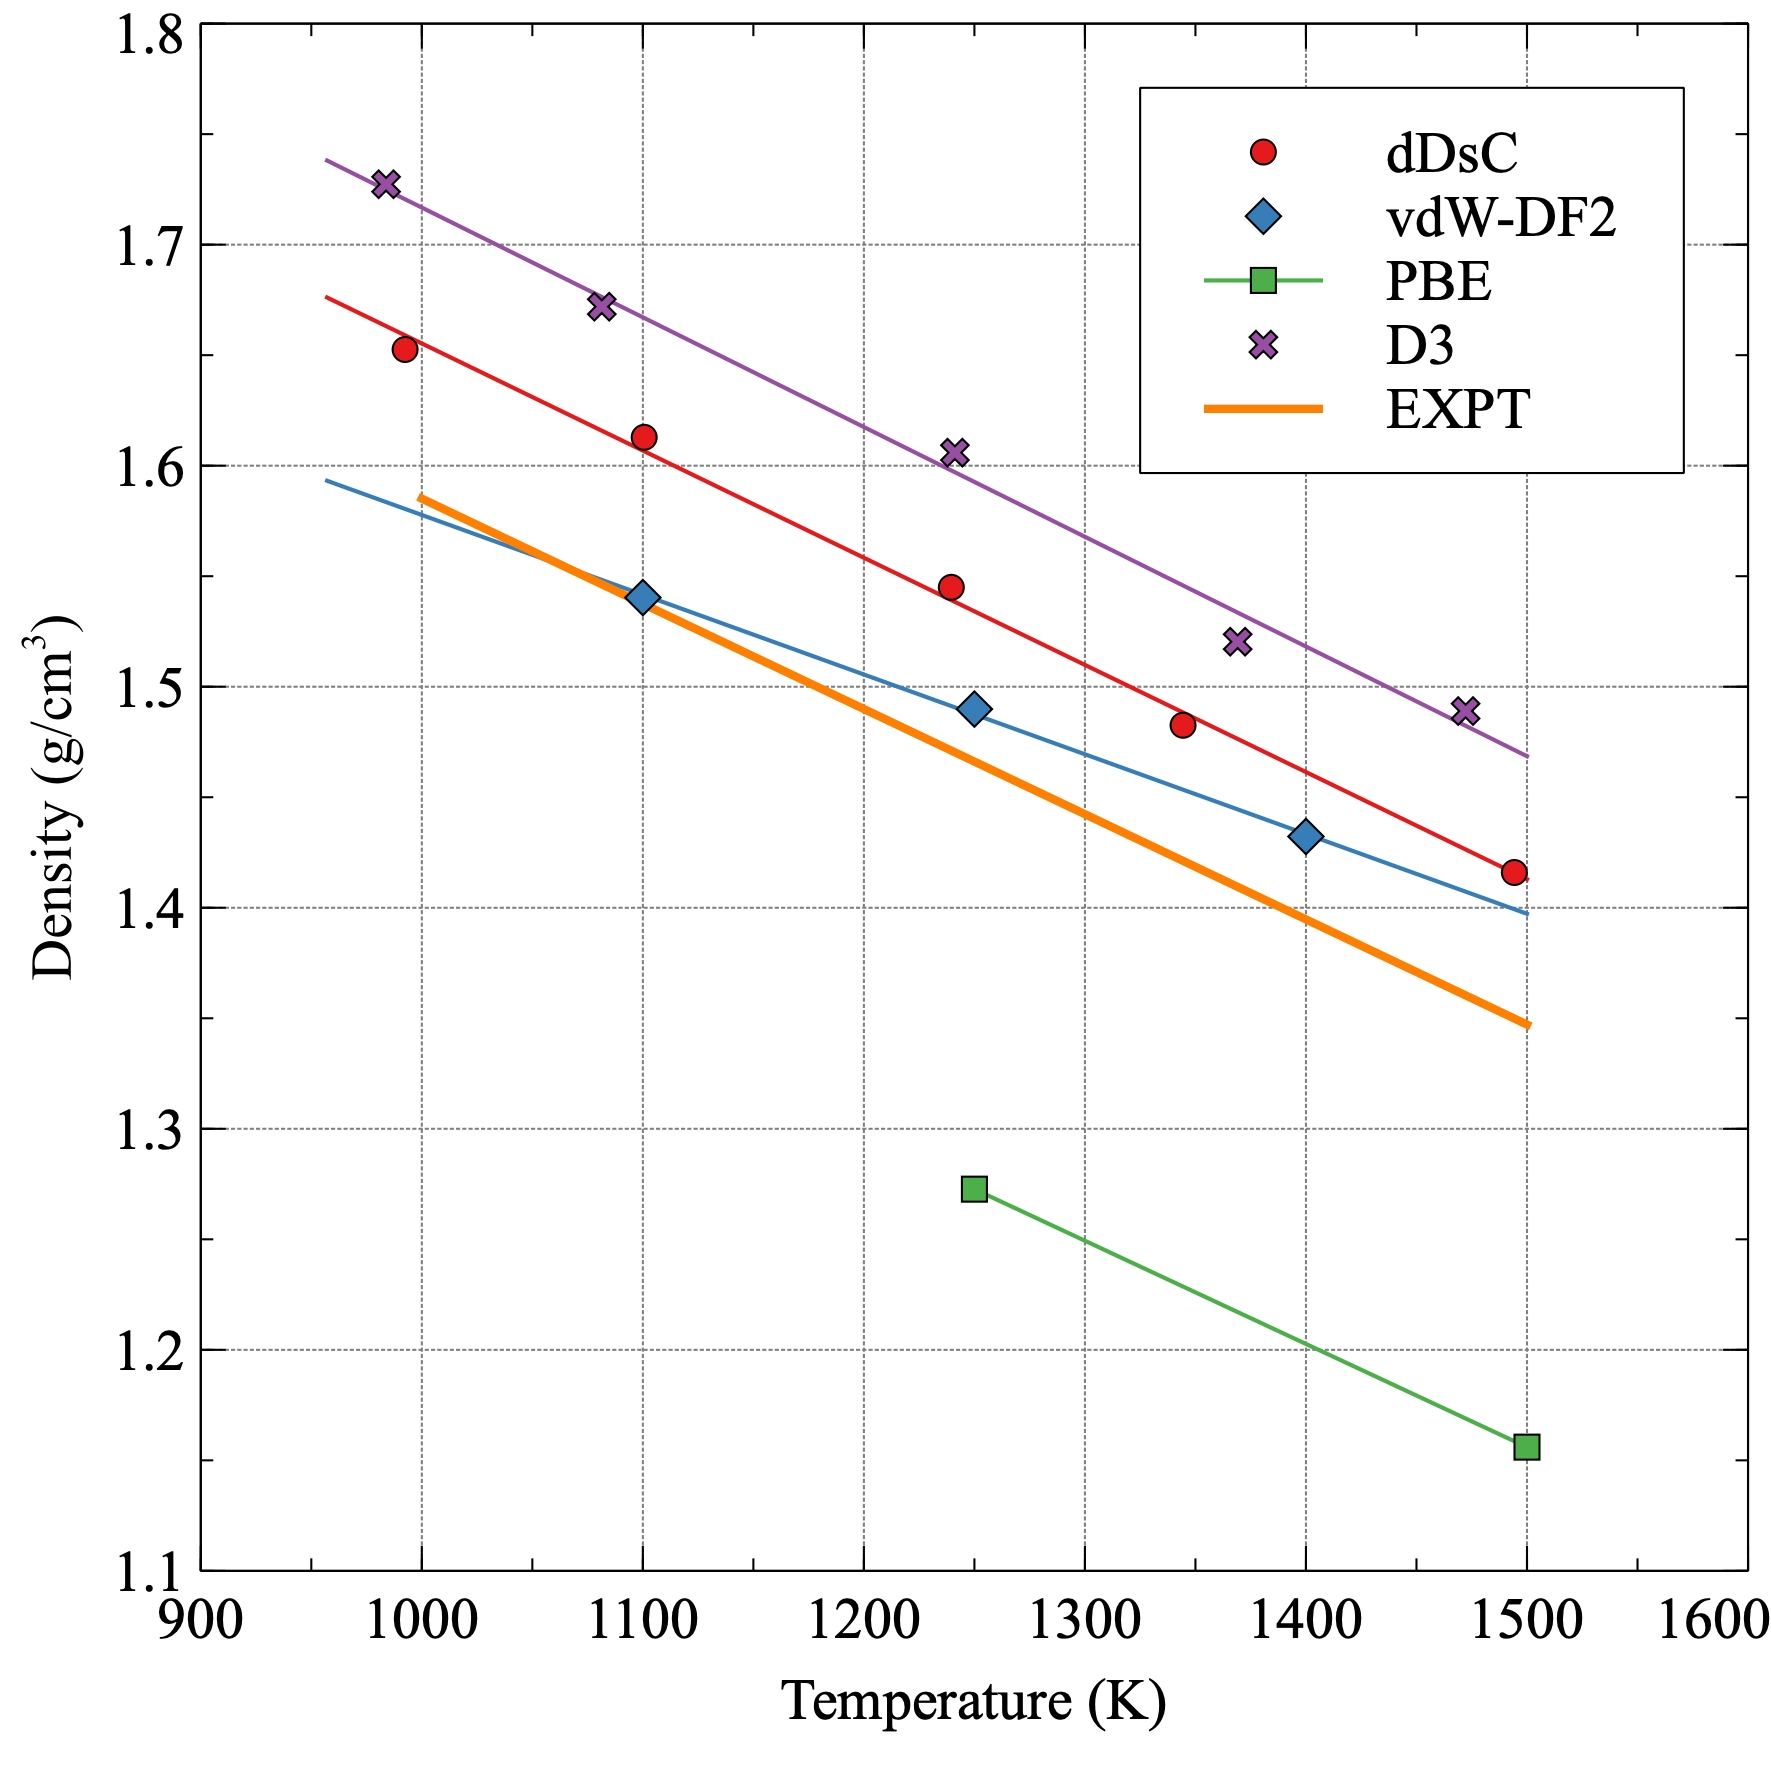
\includegraphics[width=0.6\textwidth]{fig3a.jpg}
\caption{a) Density of NaCl predicted with two different models for dispersion forces (D3 and dDsC) and one without (small cell witih 64 atoms for dDsC, large cell with 208 atoms for others). Experimental data is represented by the correlation plotted as an orange line~\cite{Janz1988}. b) Calculated total energy of NaCl as function of temperature (small cell). The line is a least-squares fit to data points and the slope represents the heat capacity.} 
%Note that the temperature range of the experimental correlation and some data points extend beyond the boiling point of NaCl, which is solely for illustrative purposes. 
%The lines shown are least-squares fits to the calculated data points.} 
\label{fig:NaCldensity}
\end{figure*}

\begin{table*}[hb!]
\centering
\begin{tabular}{lcc}
\hline
\hline
& Density (g/cm$^3$) &Heat capacity (J/mol/K) \\
%%&a &b &b \\
\hline
%NaCl Calculated (D3)	& &  \\
NaCl Calculated (dDsC)	&$2.1594-0.0004993T$ &71.6 \\
NaCl Calculated (vdW-DF2)	& 1.9379-0.0003603T & 58.1 \\
NaCl Experiment	&$2.061-0.0004759T$~\cite{Janz1988} &66.9~\cite{NIST}  \\	
UCl$_3$ Calculated (dDsC) &$6.1066-0.001383T$ &145.3 \\	
UCl$_3$ Calculated (vdW-DF2) &$4.7230-0.000554T$ & 128.5 \\	
UCl$_3$ Experiment	&$6.375-0.001522T$~\cite{Desyatnik} &150~\cite{BENES2008},129.704~\cite{YIN2020} \\
\hline
\hline
\end{tabular}
\caption{Calculated and experimental correlations and values for density and heat capacity of NaCl and UCl$_3$. For the dDsC method, the heat capacity is at constant pressure, while for the vdW-DF2 method, the heat capacity is at constant volume.}% The first quantity is a linear function of temperature, while the latter two are constants.}
\label{table:NaCldensityetc}
\end{table*}

\subsubsection{Heat capacity} 
The heat capacities are determined via equation \ref{eq:cp}, which is the slope of the total energy as a function of temperature. The constant pressure heat capacity (C$_p$) and the constant volume heat capacity (C$_V$) were obtained from the dDsC and the vdW-DF2 dispersion models, respectively, and are provided in Table \ref{table:NaCldensityetc} together with an experimental reference value~\cite{NIST}. The simulation results indicate a constant heat capacity, though in order to identify small deviations from this behavior a denser temperature mesh would be required. The good agreement between simulations and experiments for the heat capacity (see Table \ref{table:NaCldensityetc}) further emphasizes the accuracy of the AIMD simulations. The ratio of the heat capacities ($\gamma$ = C$_p$/C$_V$) is found to be 1.23, indicating a degree of compressibility, which will be discussed later. 

%Figure \ref{fig:NaCldensity}b plots the total energy per formula unit of molten NaCl as function of temperature. The derivative equals the heat capacity of NaCl, which is also tabulated in Table \ref{table:NaCldensityetc} together with an experimental reference value~\cite{NIST}. The results refer to the supercell size that we consider best converged for each methodology, see caption and below for further discussion. 

\subsubsection{Impact of supercell size and other simulation settings}
The results in Figure \ref{fig:NaCldensity} refer to simulations based on the supercell that we consider best converged. Figure \ref{fig:NaClsize} compares these results with those obtained from other supercells. Given the good agreement between the results from different supercells, density and heat capacity are considered accurately represented by all supercell sizes that were investigated.
%smaller supercells, at least below 1750 K, which supports the accuracy of the results with respect to the supercell size. 
 These results suggest that for NaCl, the larger supercells are not required to achieve converged results for density and heat capacity, which is consistent with the discussion of radial distribution functions in Sec. \ref{sec:method}. The small variations between supercells are more likely related to sampling differences, rather than due to the supercell size. Consequently, the converged results in Figure \ref{fig:NaCldensity} as well as the correlations in Table \ref{table:NaCldensityetc} are representative of all simulation results in this study, regardless of the supercell size. %Some deviation is observed for the highest temperature, which may be related to approaching the boiling temperature. 

{\color{red} I think we should add all of the supercell size discussion into the computational details. i also think only using one example, of NaCl or UCl3 would be fine.} 

\begin{figure*}[htb]
\centering
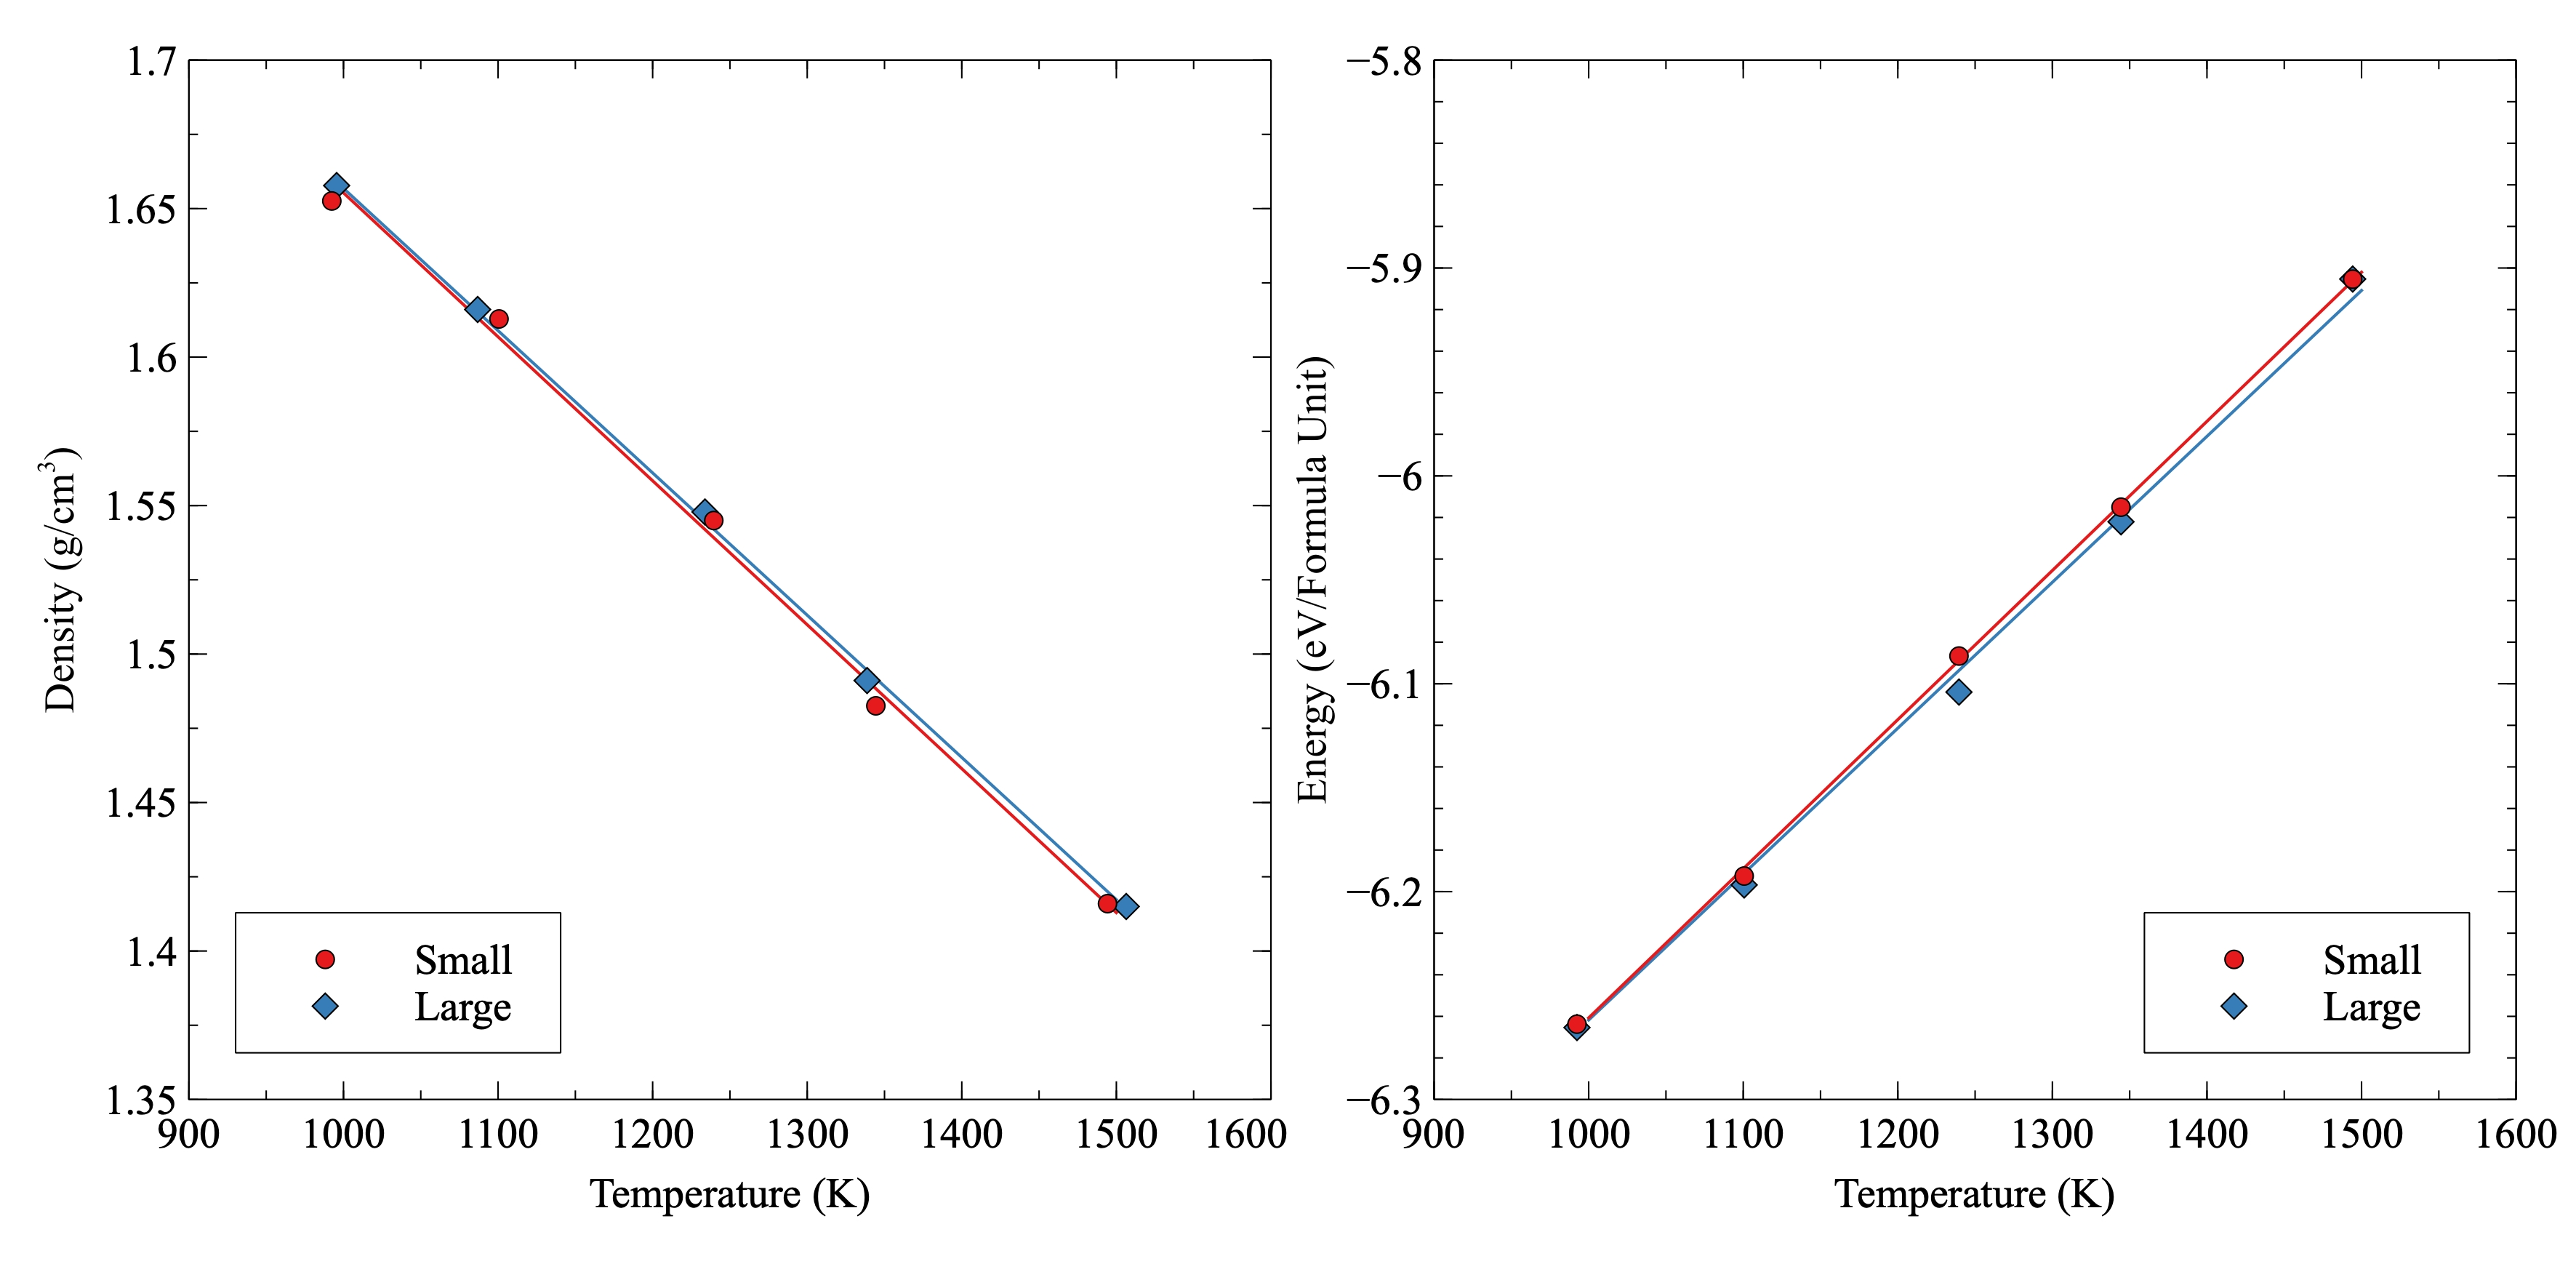
\includegraphics[width=0.9\textwidth]{fig4.jpg}
\caption{a) Calculated density and b) total energy of NaCl as function of temperature for the large and small supercells. The lines are least-squares fits to data points and the slope represents the heat capacity.} 
\label{fig:NaClsize}
\end{figure*}

%The NVT simulations also allow calculation of the compressibility and diffusivity of each species. These results are also summarized in Table \ref{table:NaCldensityetc} (compressibility) and Table \ref{table:NaCldiffusivityetc}.

\FloatBarrier

\subsection{AIMD simulations of UCl$_3$}
\subsubsection{Density and structure}
Following the results for NaCl, the best performing Van der Waals models (dDsC and vdW-DF2) were applied to UCl$_3$. Figure \ref{fig:UCl3density}a) plots the predicted density for UCl$_3$ as function of temperature for the dDsC and vdW-DF2 dispersion models compared to two literature correlations derived from experiments~\cite{Janz1988,Desyatnik}. The two experimental correlations for density are surprisingly different and cannot both be correct, except in a narrow temperature range.  The temperature dependence is predicted to be close to linear across the full temperature range investigated. The dDsC only slightly under-predicts the density and temperature dependence in the experimental data due to Desyatnik et al.~\cite{Desyatnik}. The vdW-DF2 shows a further under-prediction of the experimental densities from Desyatnik, and a further reduction in the temperature dependence. The densities in Figure \ref{fig:UCl3density} were fitted to linear correlations and summarized in Table \ref{table:NaCldensityetc}. Given the extreme disparity in the experimental literature, additional experimental efforts are encouraged to gain further certainty in the density of UCl$_3$. 


%The inset highlights the difference in energy between the AFM, FM and non-magnetic simulations. 
%Figure \ref{fig:UCl3density}b) also includes results from simulations that do not include the Hubbard $U$ model for the U 5f electrons. 
% The most recent experimental data set agrees well with the simulation data, with both the Langreth \& Lundqvist and dDsC model predicting values within a few per cent of the experimental data. 
%The Langreth \& Lundqvist methodology is sensitive to the choice of exchange -correlation potential. The optimal choice proved excellent agreement with experiments, while other choices may lead to significant underestimation of the density despite performing very well for the NaCl benchmark system. 
 %Note that only a single point was calculated for the DFT-D3 model, but that indicates essentially the same behavior as the dDsC model.  
 %Compared to the Desytniak et al. correlation~\cite{Desyatnik}, the predicted temperature dependence of the density is slightly different. 
 
 
The radial pair distribution function at 1250 K is reported in Figure \ref{fig:radial}, which highlights a first-shell coordination distance of 2.82~\AA. The coordination distance is in excellent agreement with the experimental values of 2.82 \AA~\cite{Neilson} and 2.84 \AA~\cite{Okamoto} measured at 1113 K and 1200 K, respectively, while it is higher than the AIMD simulations by Li et al.~\cite{Li}, which can likely be ascribed to the application of the Hubbard $U$ methodology in the present study. The predicted coordination numbers are within the 6 to 8 range reported in experiments and previous simulations~\cite{Li,Neilson,Okamoto}. %The U-U radial distribution function tends to zero slower than the 
 
% The effect of including the Hubbard $U$ model is to decrease the density (increase the volume) compared to the reference case, which is consistent with the increase in volume observed for solid state simulations using the Hubbard $U$ methodology. The results without the Hubbard $U$ parameter is slightly closer to the densities measured in experiments. The magnetic order has a very small influence on the predicted density, which is highlighted in Figure \ref{fig:UCl3density}b). %We believe that the AFM (random) distribution is more representative of the high-temperature behavior of molten salts, as it should exhibit the lowest free energy (see below).

\begin{figure*}[htb]
\centering
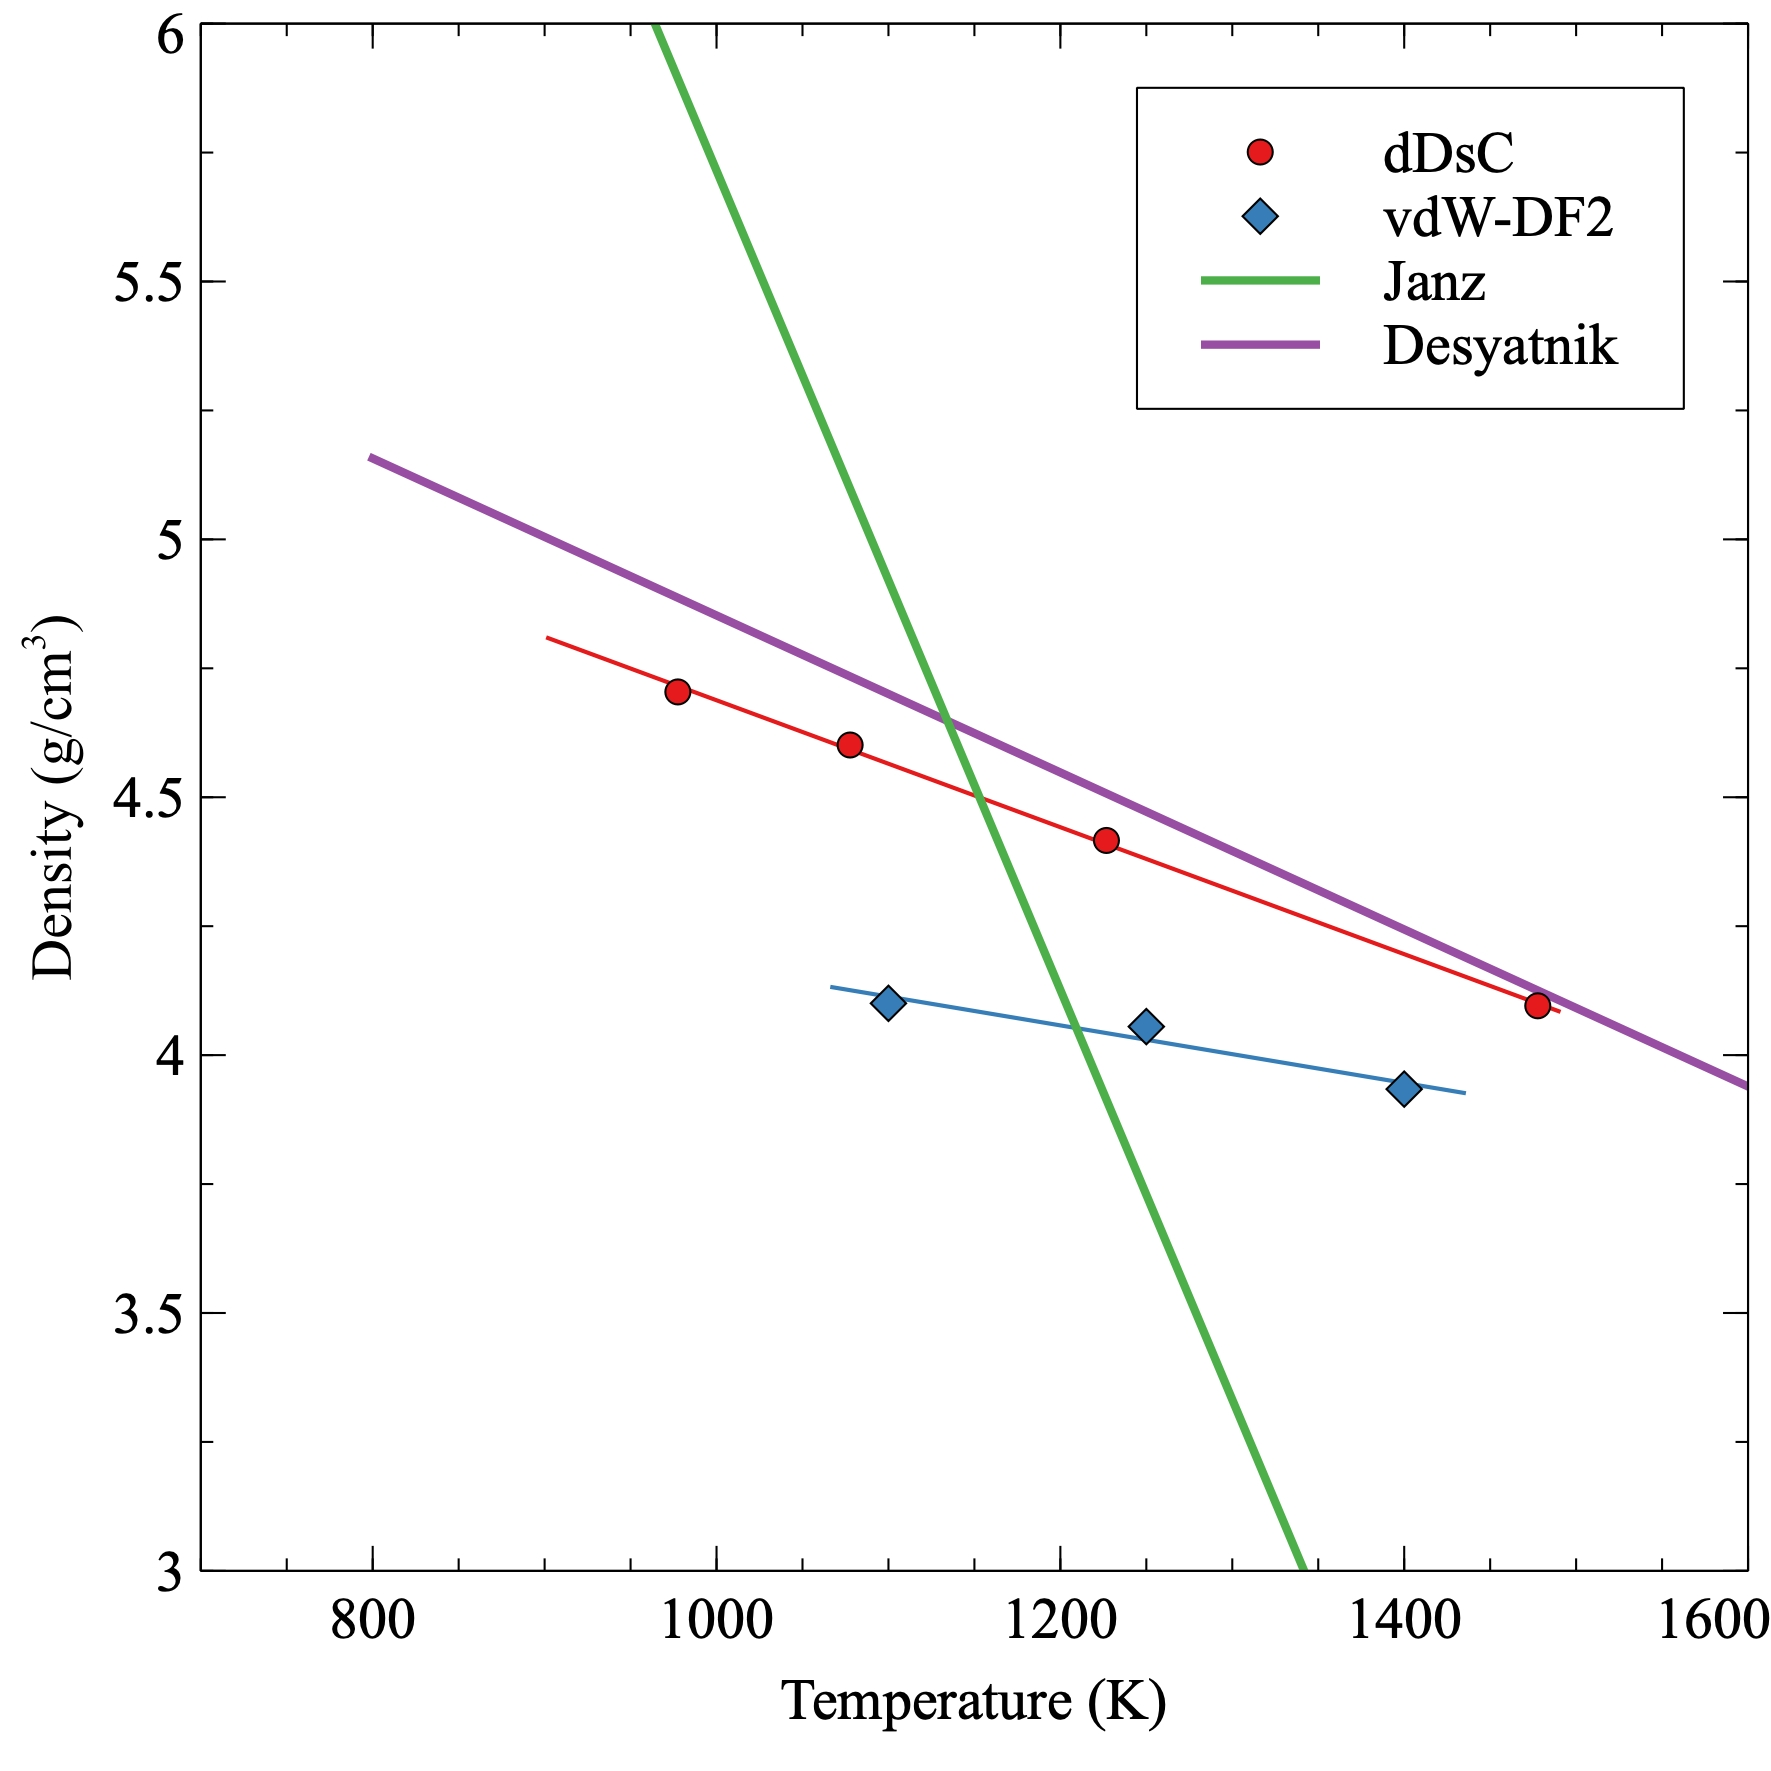
\includegraphics[width=0.5\textwidth]{fig5.jpg}
\caption{a) Density of UCl$_3$ predicted the dDsC model for the dispersion forces (small cell with 64 atoms). Experimental data is represented by the correlations plotted as green~\cite{Desyatnik} and orange lines~\cite{Janz1988}. The dashed line is a least-squares fit to the calculated data points, the equations of which are summarized in Table \ref{table:NaCldensityetc}. b) Calculated total energy of UCl$_3$ as function of temperature (small cell). The line is a least-squares fit to data points and the slope represents the heat capacity.} 
\label{fig:UCl3density}
\end{figure*}

\subsubsection{Heat capacity} 
%Figure \ref{fig:UCl3density} plots the total energy as function of temperature, from which the heat capacity can be derived by calculating the slope. The total energy closely follows a linear relation as function of temperature and, consequently, the heat capacity can be approximated as a constant in the temperature range investigated. In order to resolve small deviations from the linear relation, a denser temperature mesh would have to be used. 
%Experimental data for the heat capacity of UCl$_3$ has not been identified, but our results compare very well with the value derived from the CALPHAD assessment of the UCl$_3$ thermodynamics due to Benes et al.~\cite{BENES2008}, while it deviates somewhat from the assessment due to Yin et al.~\cite{YIN2020} (see Table~\ref{table:NaCldensityetc}). %Figure \ref{fig:fig:UCl3heat}b compares the total energy as function of temperature for simulations assuming different magnetic ordering. The AFM (random) ordering is predicted to be slightly more stable than the FM ordering, though the difference is small. The AFM (random) model would be further stabilized by the magnetic entropy originating from the random distribution of magnetic moments at finite temperature. Consequently, the AFM (random) distribution of magnetic moments is considered to be the most representative model. %, which confirms AFM (random) ordering as the most appropriate model for production simulations. 

%\begin{figure}[htb]
%\centering
%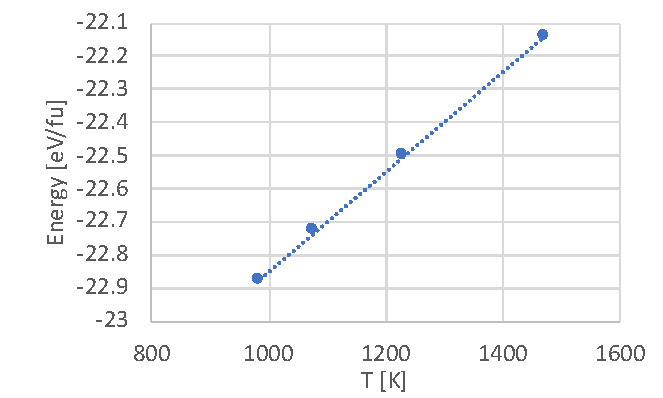
\includegraphics[width=0.95\textwidth]{FIG5.pdf}
%\caption{Calculated total energy of UCl$_3$ as function of temperature (small cell). The line is a least-squares fit to data points and the slope represents the heat capacity.} 
%\label{fig:UCl3heat}
%\end{figure}

The heat capacities are determined as the slope of the total energy as a function of temperature. The total energy closely follows a linear relation as function of temperature and, consequently, the heat capacity can be approximated as a constant in the temperature range investigated. In order to resolve small deviations from the linear relation, a denser temperature mesh would have to be used. The constant pressure heat capacity (C$_p$) and the constant volume heat capacity (C$_V$) were obtained from the dDsC and the vdW-DF2 dispersion models, respectively, and are provided in Table \ref{table:NaCldensityetc}. Experimental data for the heat capacity of UCl$_3$ has not been identified, but our results compare very well with the value derived from the CALPHAD assessment of the UCl$_3$ thermodynamics due to Benes et al.~\cite{BENES2008}, while it deviates somewhat from the assessment due to Yin et al.~\cite{YIN2020}. The ratio of the heat capacities ($\gamma$ = C$_p$/C$_V$) is found to be 1.15, indicating a lesser degree of compressibility than for the NaCl system. 

{\color{red} I removed the plot of the heat capacity, as it only shows a single line, which is not especially enlightening. if you want to add it back in, we can do so.}

\subsubsection{Impact of supercell size and other simulation settings}
The results discussed above for UCl$_3$ refer to simulations using the supercell size that we deem to be best converged and most representative of the UCl$_3$ system for each simulation methodology. Select results obtained from different supercell sizes are compared in Figure \ref{fig:UCl3size}, which exhibits fairly good agreement with each other. Any difference between supercell sizes is primarily ascribed to sampling appropriate configurations rather than an effect of increasing the numbers of ions in the simulation box, although additional simulations would be required to fully certify this conclusion. Compared to NaCl it is much more challenging to reach long simulation times for the large UCl$_3$ simulation cells. 

{\color{red} As I mentioned, I think the supercell size stuff should all go in the methods}

\begin{figure*}[htb]
\centering
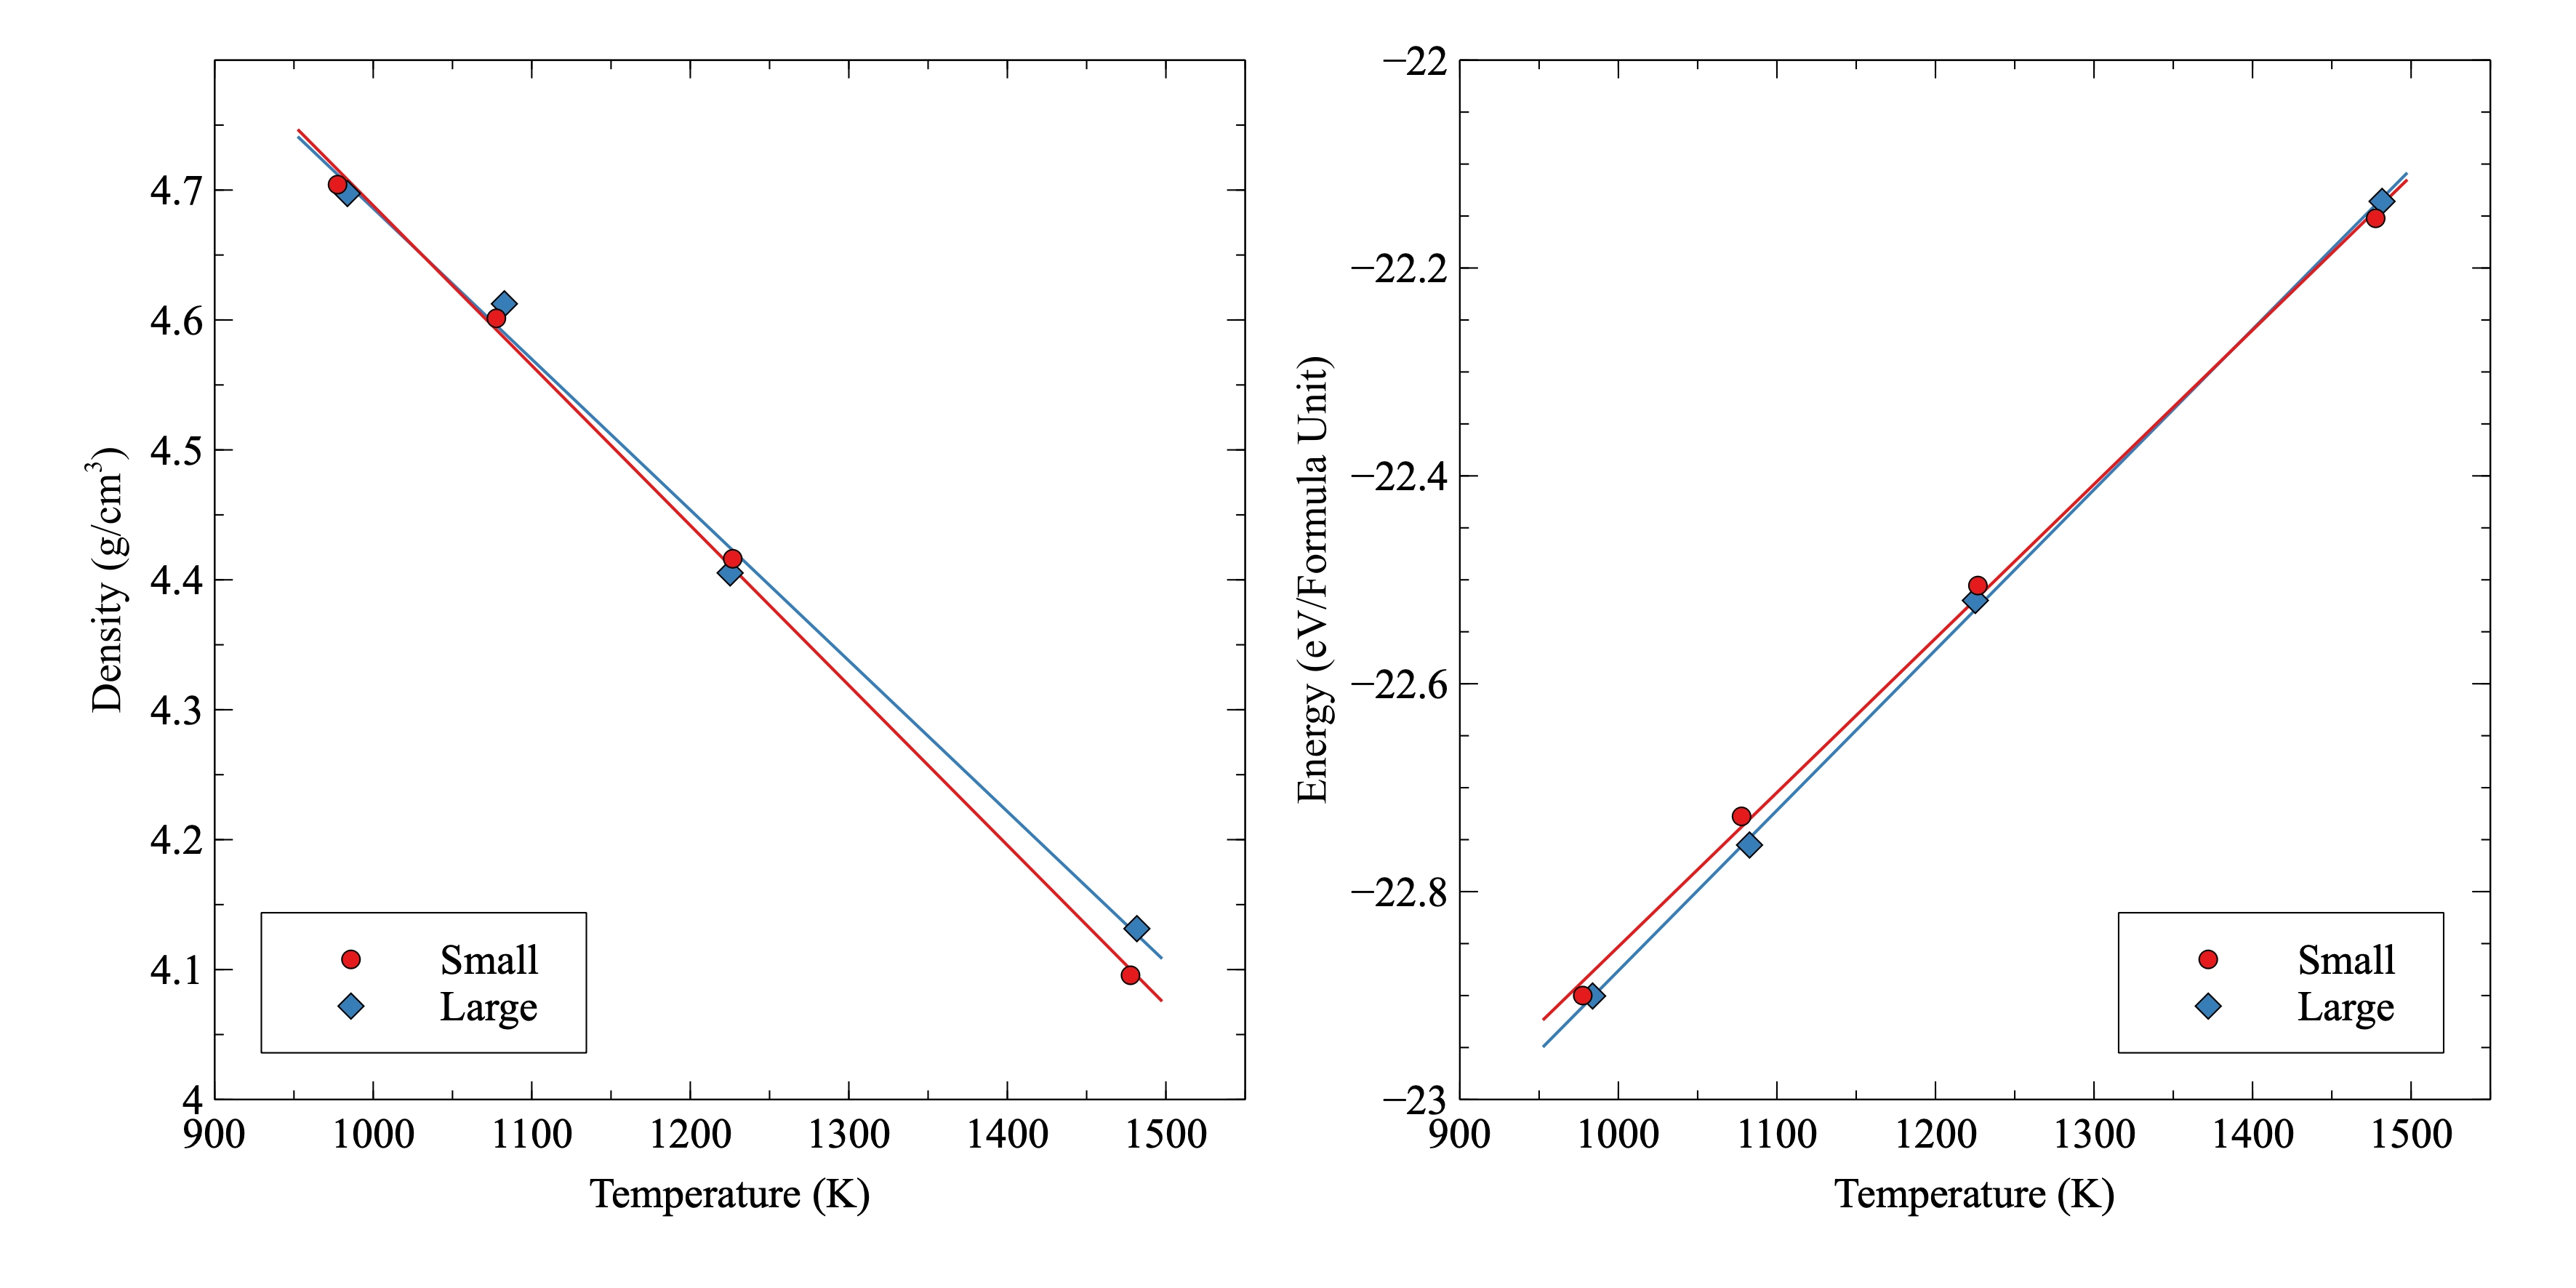
\includegraphics[width=0.9\textwidth]{fig6.jpg}
\caption{Calculated density and total energy of UCl$_3$ as function of temperature for the large and small supercells. The line is a least-squares fit to data points and the slope represents the heat capacity.} 
\label{fig:UCl3size}
\end{figure*}

\FloatBarrier

\subsection{Ab initio molecular dynamics simulations on NaCl-UCl$_3$}
\subsubsection{Density and structure}
The density of NaCl-UCl$_3$ mixtures were calculated for the dDsC and the vdW-DF2 dispersion model at three or four (depending on composition) different temperatures between 900 K and 1500 K, as shown in Figure \ref{fig:NaClUCl3}a). This figure also includes densities at the same temperatures as those of the simulations obtained from Redlich-Kister (RK) correlations \cite{agca2022} derived from experimental data due to Desyatnik et al.~\cite{Desyatnik}. The simulated data points are generally within a few per cent of the experimental data. 

\begin{figure*}[htb]
\centering
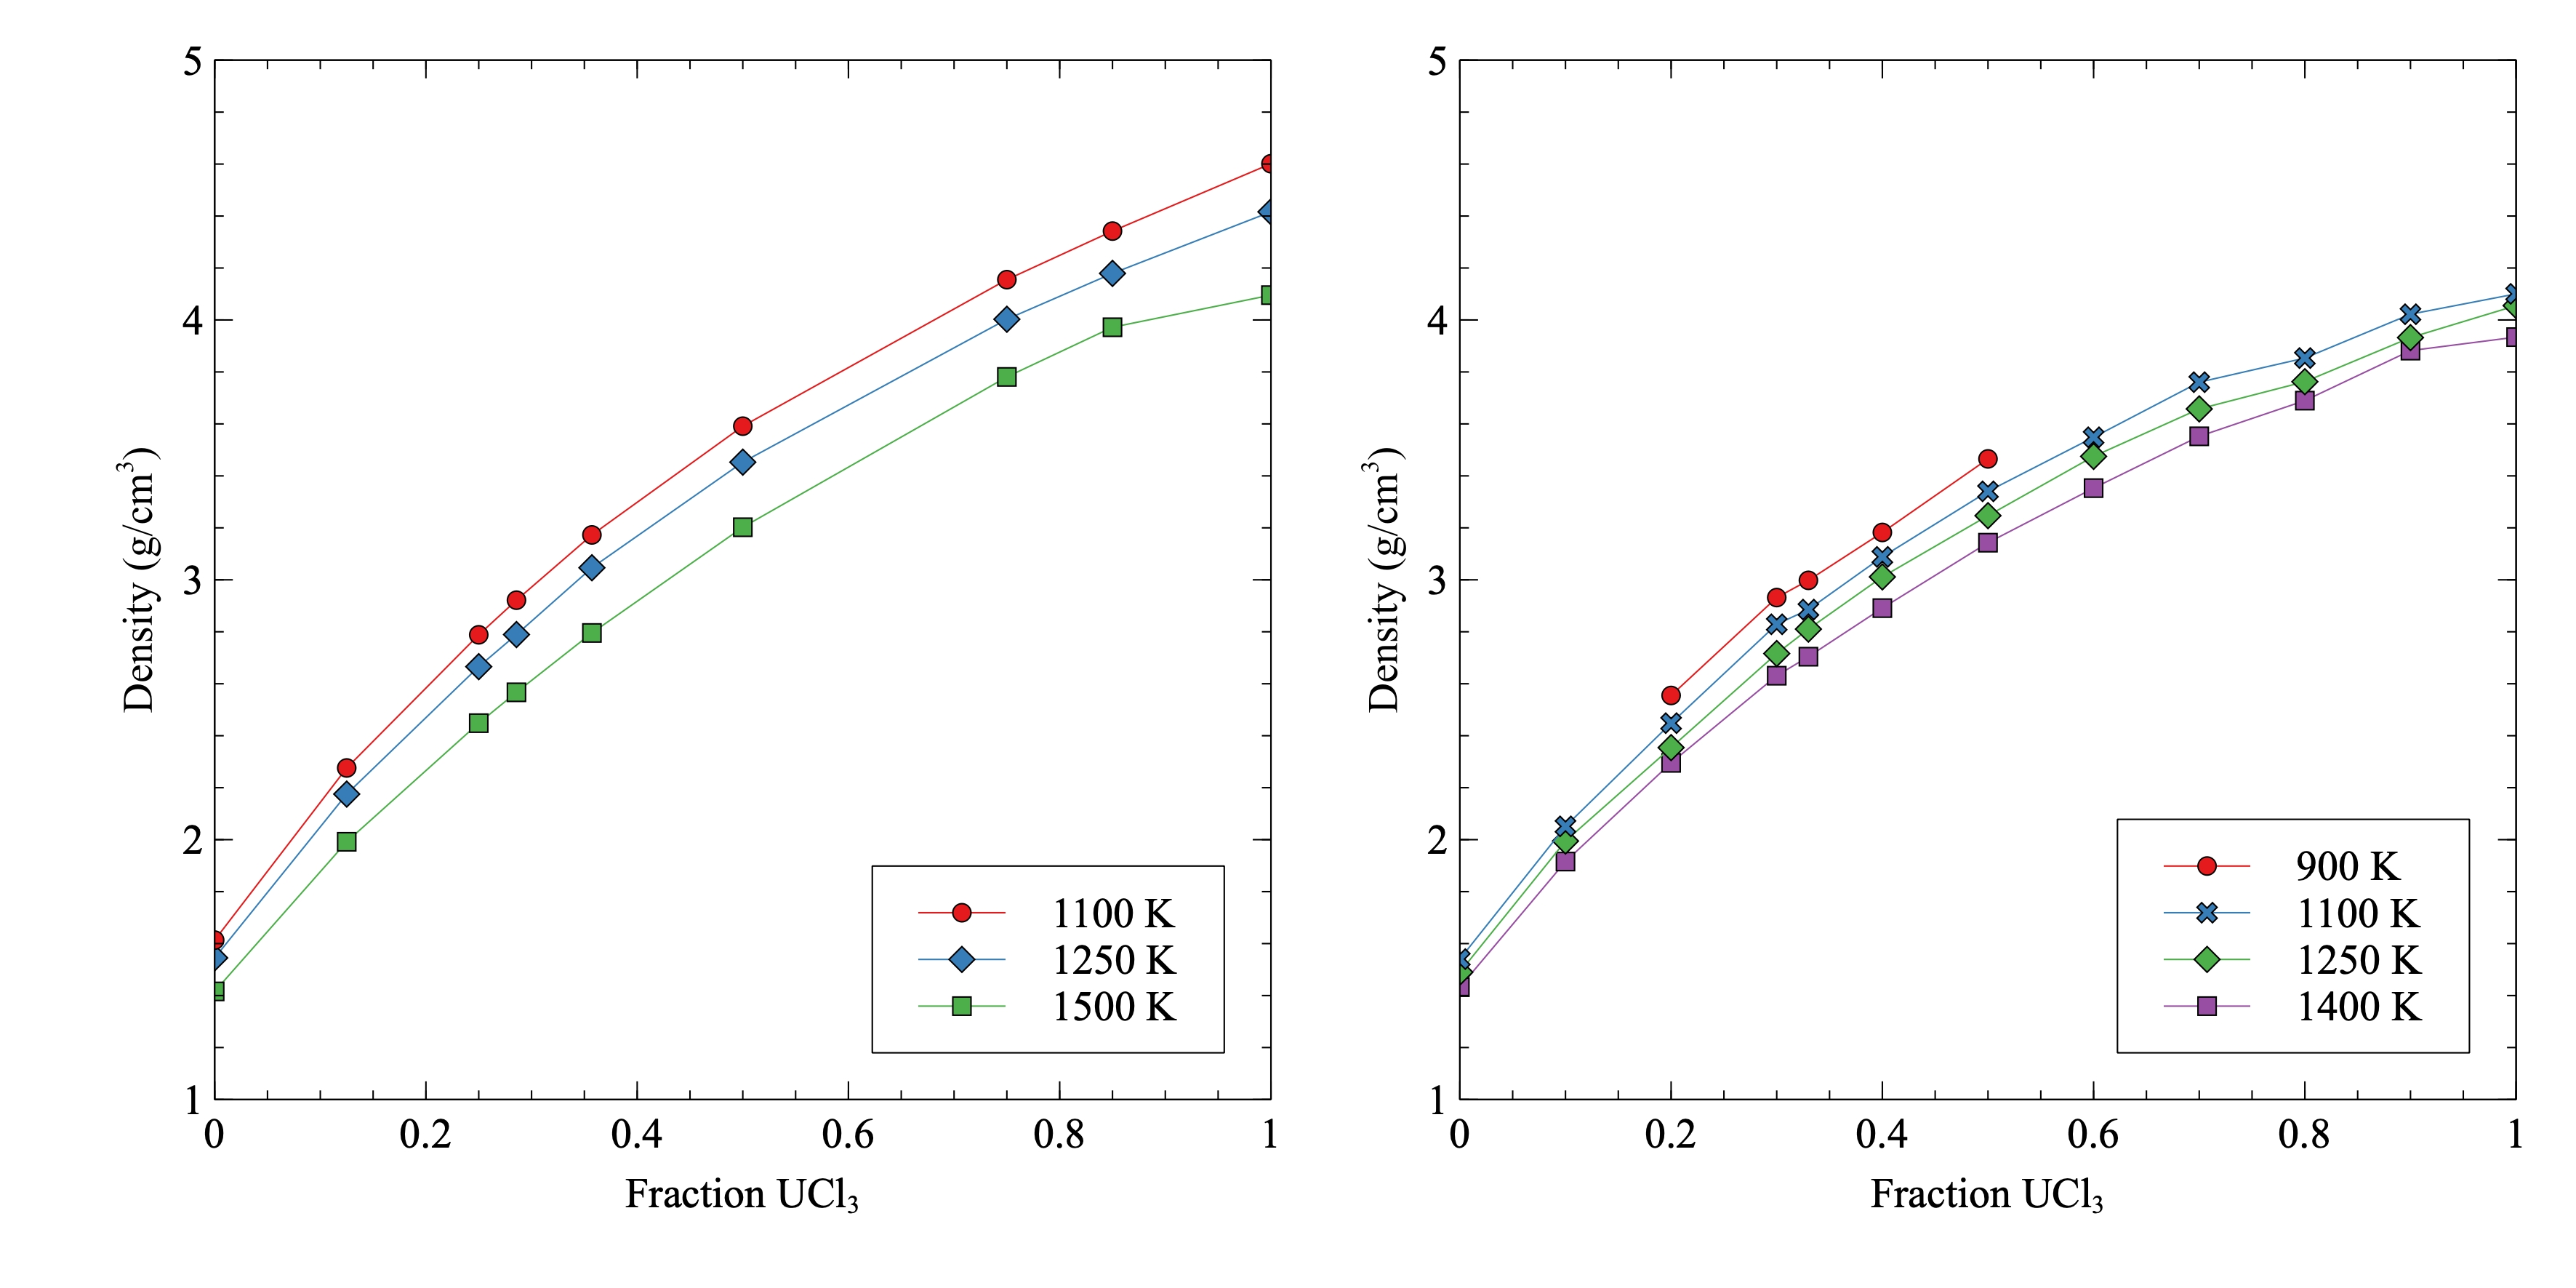
\includegraphics[width=0.9\textwidth]{fig7.jpg}
\caption{Density of NaCl-UCl$_3$ mixtures as obtained from simulations using the (a) dDsC dispersion formulation, and (b) the vdW-DF2 dispersion formulation at temperatures between 900 K and 1500 K. The solid lines represent the Redlich-Kister correlation to the Desyatnik \cite{Desyatnik} data from Agca \cite{agca2022}.%The lines represent an ideal solution with the calculated and experimental NaCl and UCl$_3$ densities as end points. 
%b) The fractional deviation form ideal solution behavior plotted as function of composition at temperatures between 1100 K and 1500 K. %Results for both the large and small supercells are shown.
} 
\label{fig:NaClUCl3}
\end{figure*}

The deviation from ideal mixing for the dDsC dispersion is shown in Figure \ref{fig:ideal} and compared to the experimental deviation from ideal mixing from Desyatnik \cite{Desyatnik}. Figure \ref{fig:ideal} highlights the fractional deviation from ideal solution behavior as calculated from simulations and experiments~\cite{agca2022,Desyatnik}. It is challenging to converge the density for mixed salt solutions to an accuracy better than around one per cent of the absolute density using AIMD simulations, which gives rise to some scatter in the data points. Nevertheless, a few trends are discernible from Figure \ref{fig:NaClUCl3}. The simulations suggest a negative deviation from an ideal solution (lower density than predicted by an ideal solution behavior) by up to 2-3\%, except close to pure UCl$_3$ at high temperature where a positive deviation is observed. According to our simulations, the magnitude of the deviation from ideal solution behavior is a function of composition and varies some with temperature starting at $x\approx0.35$ and continuing in the UCl$_3$ rich composition range, while it is almost independent of temperature in the NaCl rich range. 
The maximum deviation from ideal solution behavior occurs close to the eutectic composition of 35\% UCl$_3$, perhaps slightly shifted towards the NaCl rich side but it is hard to draw a solid conclusion due to uncertainties in the simulated data. These predictions are qualitatively similar to the correlations derived from experiments by Desyatnik et al.~\cite{Desyatnik}, though the experimental correlations predict a larger magnitude for the deviation from an ideal solution and also exhibit a stronger temperature dependence than the simulations. 

\begin{figure*}[htb]
\centering
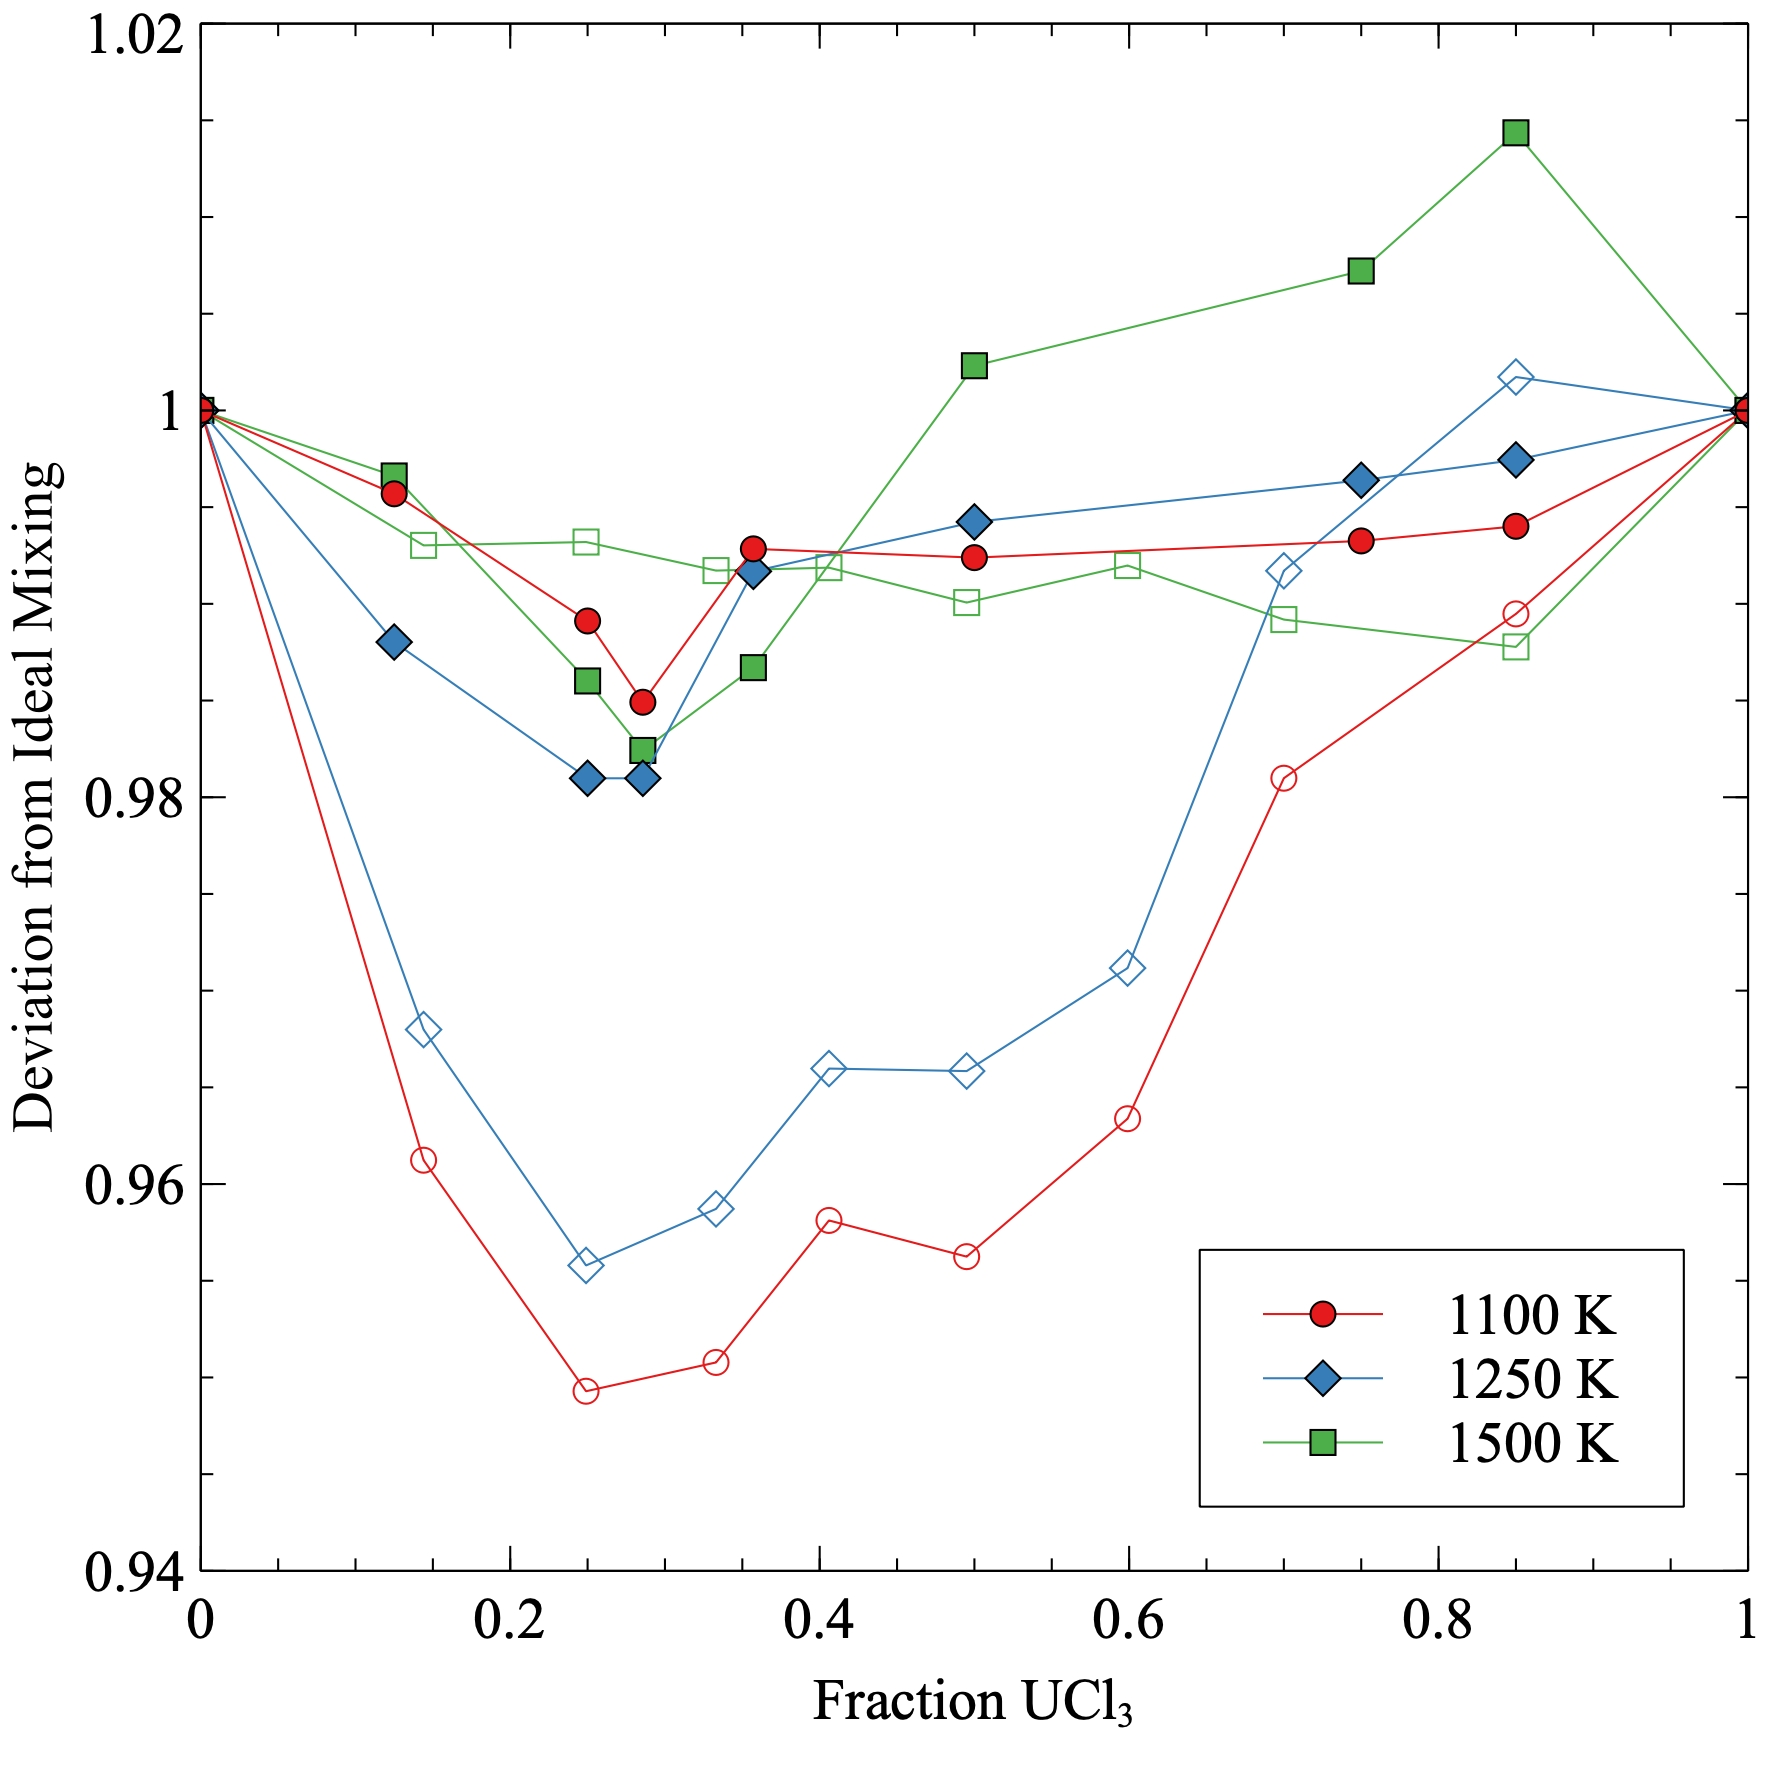
\includegraphics[width=0.5\textwidth]{fig8.jpg}
\caption{The fractional deviation form ideal solution behavior plotted as function of composition at temperatures between 1100 K and 1500 K. The solid symbols represent the simulation data and the open symbols represent the experimental data from Desyatnik \cite{Desyatnik}.}  
\label{fig:ideal}
\end{figure*}

The density as a function of temperature displays a linear dependence for all compositions, with a unique slope at each given composition, similar to the pure end-members. The coefficients describing the linear dependence on temperature for each composition are plotted in Figure \ref{fig:TandCp}. Although there is some scatter, a weak non-linear dependence on composition for both the linear and constant term (not shown) is identified. The non-linear dependence is most pronounced in the UCl$_3$ rich range. The density correlations identified in Figures \ref{fig:NaClUCl3}, \ref{fig:ideal}, and \ref{fig:TandCp} can also be expressed in a combined composition-temperature dependent correlation:
\begin{equation}
\begin{split}
\rho(x,T)=\frac{M_{NaCl}(1-x)+M_{UCl_3}x}{\frac{M_{NaCl}(1-x)}{\rho_{NaCl}}+\frac{M_{UCl3}x}{\rho_{UCl_3}}}+ e_1+e_2T+(f_1+f_2T)x 
%(g_1+g_2T)x^2+(h_1+h_2T)x^3+(i_1+i_2T)x^4+(j_1+j_2T)x^5,
\label{eq:LS}
\end{split}
\end{equation}
{\color{red} It seems they are only needing to go to the first order in terms of temperature dependence}

where the first term represents the density of an ideal solution and the subsequent terms the deviation from ideal solution behavior. $M_{NaCl}$ and $M_{UCl_3}$ are the molar masses of the end member salts, $\rho_{NaCl}$ and $\rho_{UCl_3}$ the temperature dependent densities of the end-member salts, which are taken from the correlations previously derived, $T$ is temperature and $x$ is the mole fraction of UCl$_3$ in the mixture. This is an identical formulation to the Redlich-Kister formulation from Agca \cite{agca2022}. A least-squares fit of the coefficients describing deviation from an ideal solution are collected in Table \ref{table:LS}.
%, in principle, be used for calculating densities at temperatures and compositions not explicitly investigated by AIMD simulations. % according to the following equations,
%This approach is utilized to compare the AIMD predictions to the recent experimental data from Scott et al.~\cite{} in Fig. \ref{fig:NaClUCl3_comp} collected at XX and YY K. These experiments suggest that the density behaves much closer to an ideal solution than those due to Desyatnik et al.~\cite{}. The agreement with the AIMD predictions is still very good, considering uncertainties associated with both experiments and simulations.  

\begin{figure*}[htb]
\centering
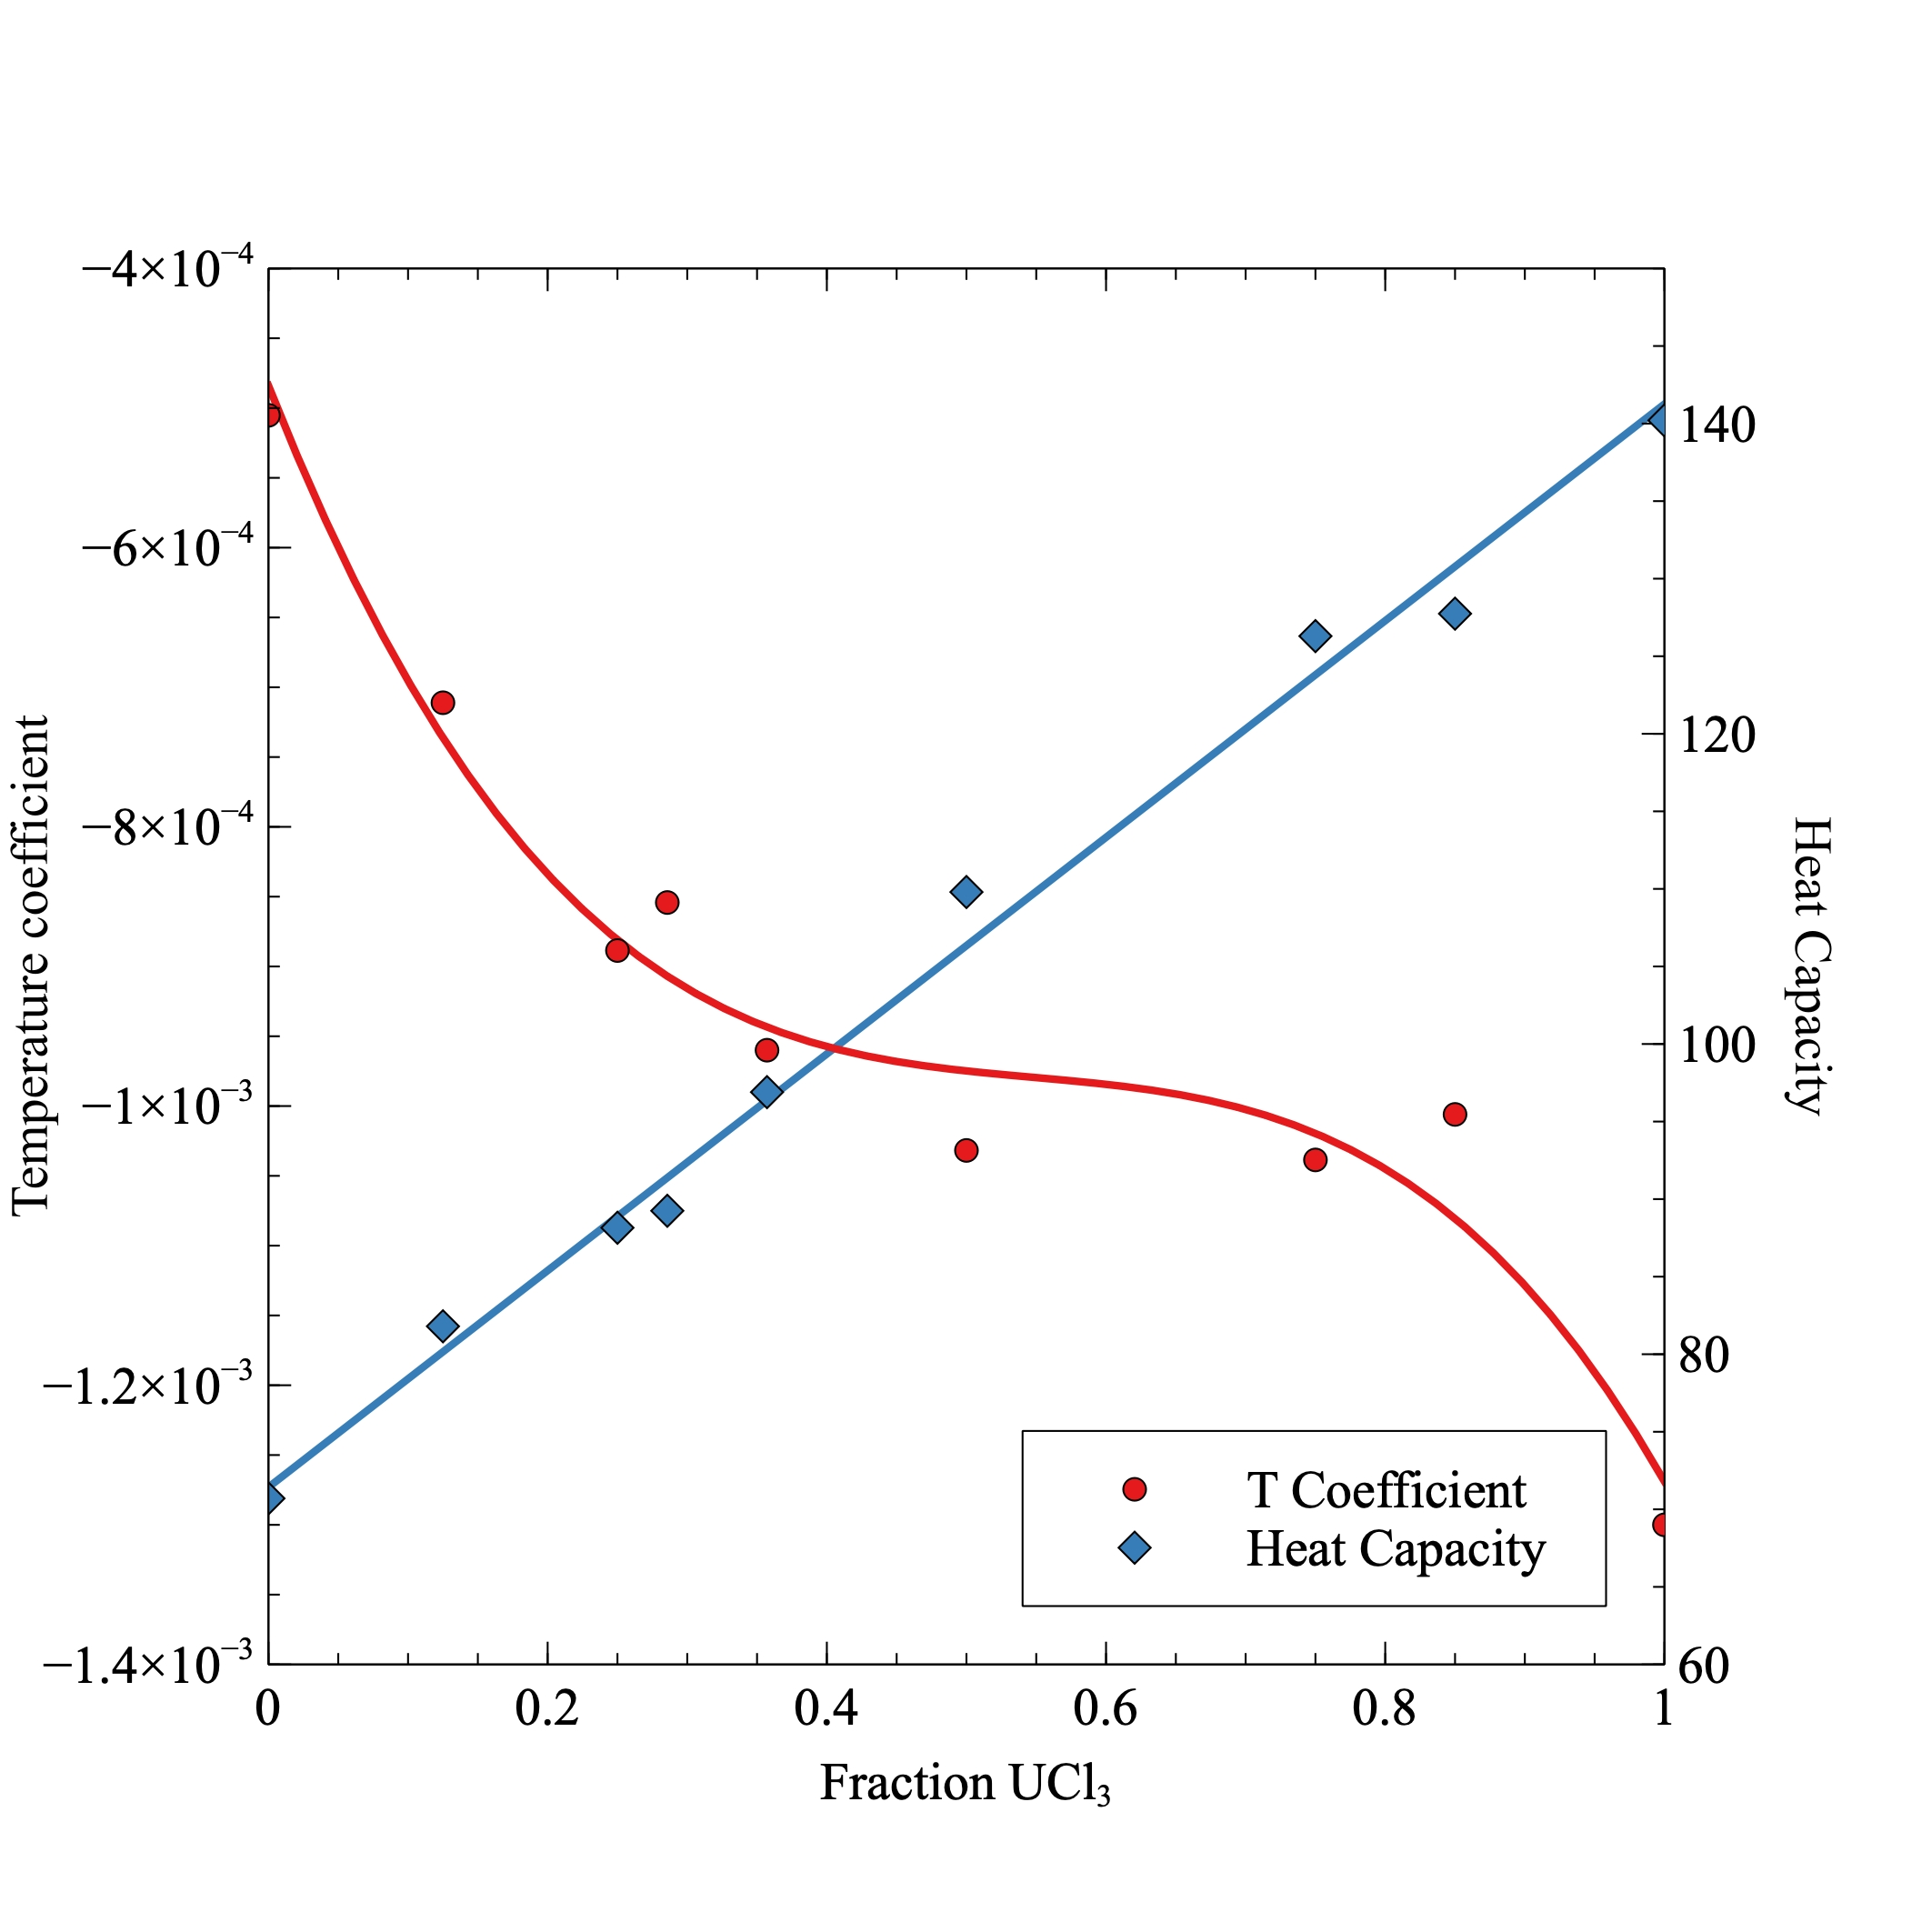
\includegraphics[width=0.6\textwidth]{fig9.jpg}
\caption{The coefficient describing the linear temperature dependence of density, and the heat capacity as function of the UCl$_3$ fraction. The solid line for the temperature coefficient represents a least-squares fit of a third order polynomial. The solid line for the heat capacity represents a least-squares fit of a linear correlation.}
\label{fig:TandCp}
\end{figure*}

%\begin{figure*}[htb]
%\centering
%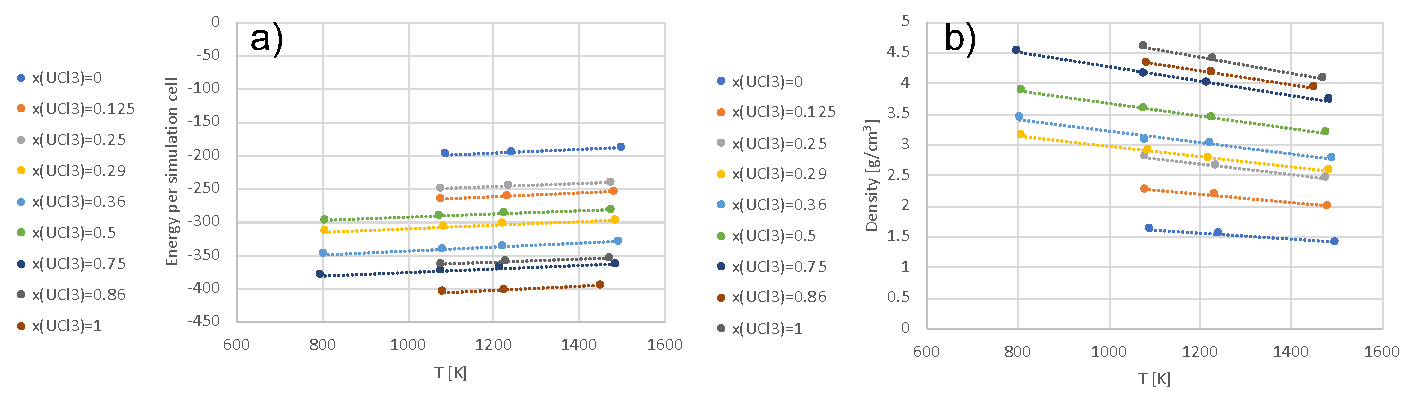
\includegraphics[width=0.95\textwidth]{FIG6c.pdf}
%\caption{a) Calculated temperature dependent densities as function of composition. b) Calculated energies per simulations cell as function of composition. In both a) and b) the lines represent least-squares fits to the calculated data.}  
%\label{fig:NaClUCl3_t}
%\end{figure*}

%\begin{figure*}[htb]
%\centering
%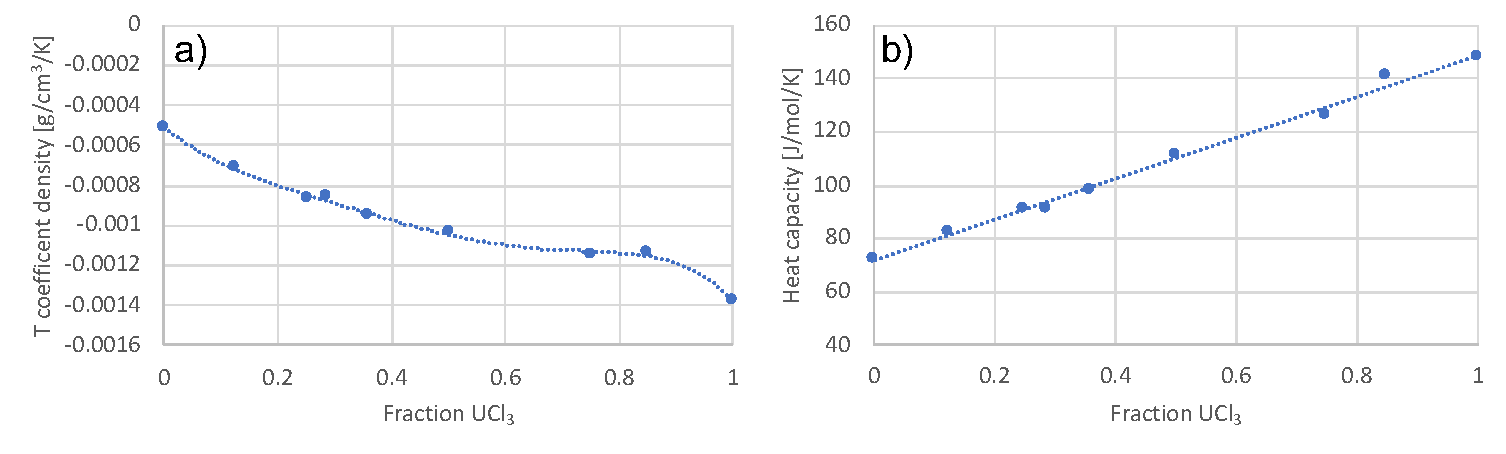
\includegraphics[width=0.95\textwidth]{FIG6f.pdf}
%\caption{a) Coefficient describing the linear temperature dependence of density as function of the UCl$_3$ fraction. The line represents a least-squares fit of a fifth order polynomial. b) Heat capacity as function of the UCl$_3$ fraction. The line represents a least-squares fit of a linear correlation.}
%\label{fig:NaClUCl3_comp}
%\end{figure*}

\begin{table*}[hb!]
\centering
\begin{tabular}{lcccccccccccc}
\hline
\hline
&$e_1$ &$e_2$ &$f_1$ &$f_2$ &$g_1$ &$g_2$ &$h_1$ &$h_2$ &$i_1$ &$i_2$ &$j_1$ &$j_2$ \\
\hline
\hline
\end{tabular}
\caption{A least-squares fit of the coefficients describing density of NaCl-UCl$_3$ mixtures as function of temperature, see Eq. \ref{eq:LS}.}% The first quantity is a linear function of temperature, while the latter two are constants.}
\label{table:LS}
\end{table*}

\FloatBarrier

\subsubsection{Heat Capacity and Mixing Energy}
The total energy for each NaCl-UCl$_3$ composition displays a linear dependence as a function of temperature, similar to the pure NaCl and UCl$_3$ systems. The heat capacity for each composition can be obtained from the slope of the total energy versus temperature, and this heat capacity is displayed in Figure \ref{fig:TandCp}. The heat capacity displays a monotonic increase with composition that exhibits an ideal mixing type behavior. Thus, for a given composition of the pseudo-binary salt, a linear interpolation of the heat capacities is an appropriate approximation. 

The mixing energies of NaCl-UCl$_3$ at temperatures ranging from 1100 K to 1500 K as calculated by the dDsC dispersion formulation are plotted in Figure \ref{fig:mixing}, with the NaCl and UCl$_3$ end members as reference points. The mixtures exhibit a negative deviation from ideal solution behavior, which implies that the solution phase is favored over a two-phase mixture of the end-points. 
{\color{red} i removed the free energy graph. let me know if i should put it back in.}
%Addition of entropy further stabilizes the mixed solution phase, as shown in Figure ref{fig:mixing} by adding a simple ideal solution model to the potential energy in Figure ref{fig:mixing}.
 The minimum (most negative) mixing energy is between $x$=0.35 and $x$=0.5, which qualitatively mimics the results for the density, perhaps with a slight shift towards the 50-50 composition. %The potential energy minimum may be shifted slightly closer to the 50-50 composition. However, it may be questionable if the simulations are sufficiently converged to draw such a subtle conclusion.  The Langreth \& Lundqvist and dDsC simulations predict very similar solution energies. The minimum of the free energy is shifted close to the 50-50 composition. 
 
 The mixing energy was measured at 1100 K by Matsuura et al.~\cite{Matsuura} and the results are also shown in Figure \ref{fig:mixing} and indicate very good agreement with the simulations across the full temperature range. In addition to the experimental data points, there are two sets of thermodynamic models for the solution energy~\cite{BENES2008,YIN2020}, and the correlation from Ref.~\cite{YIN2020} is included in Figure \ref{fig:mixing}. Both thermodynamic models assume the solution energy to be independent of temperature, which is in good agreement with the simulations. The model by Yin et al.~\cite{YIN2020} was derived from the experimental measurements by Matsuura et al.~\cite{Matsuura} and consequently agree similarly well with our simulation results. The model by Benes et al.~\cite{BENES2008} exhibits a smaller mixing energy than both the experimental data points and our simulations, but is not shown in Figure \ref{fig:mixing}. 

%Although the simulations were run long enough to sample the configuration space, it is possible that the initial distribution of Na and U ions have some impact on the results, especially for the large supercells.  In order to test this possibility, a few of the Na And Cl atoms in the previous simulations were swapped and the simulations were re-run. In particular we target the compositions that seemed to deviate from the overall trend somewhat. Indeed, the new simulations provided slightly different results in closer agreement with the trends already discussed. For the large cells, this is an inherent uncertainty of the simulation apporach.

\begin{figure*}[htb]
\centering
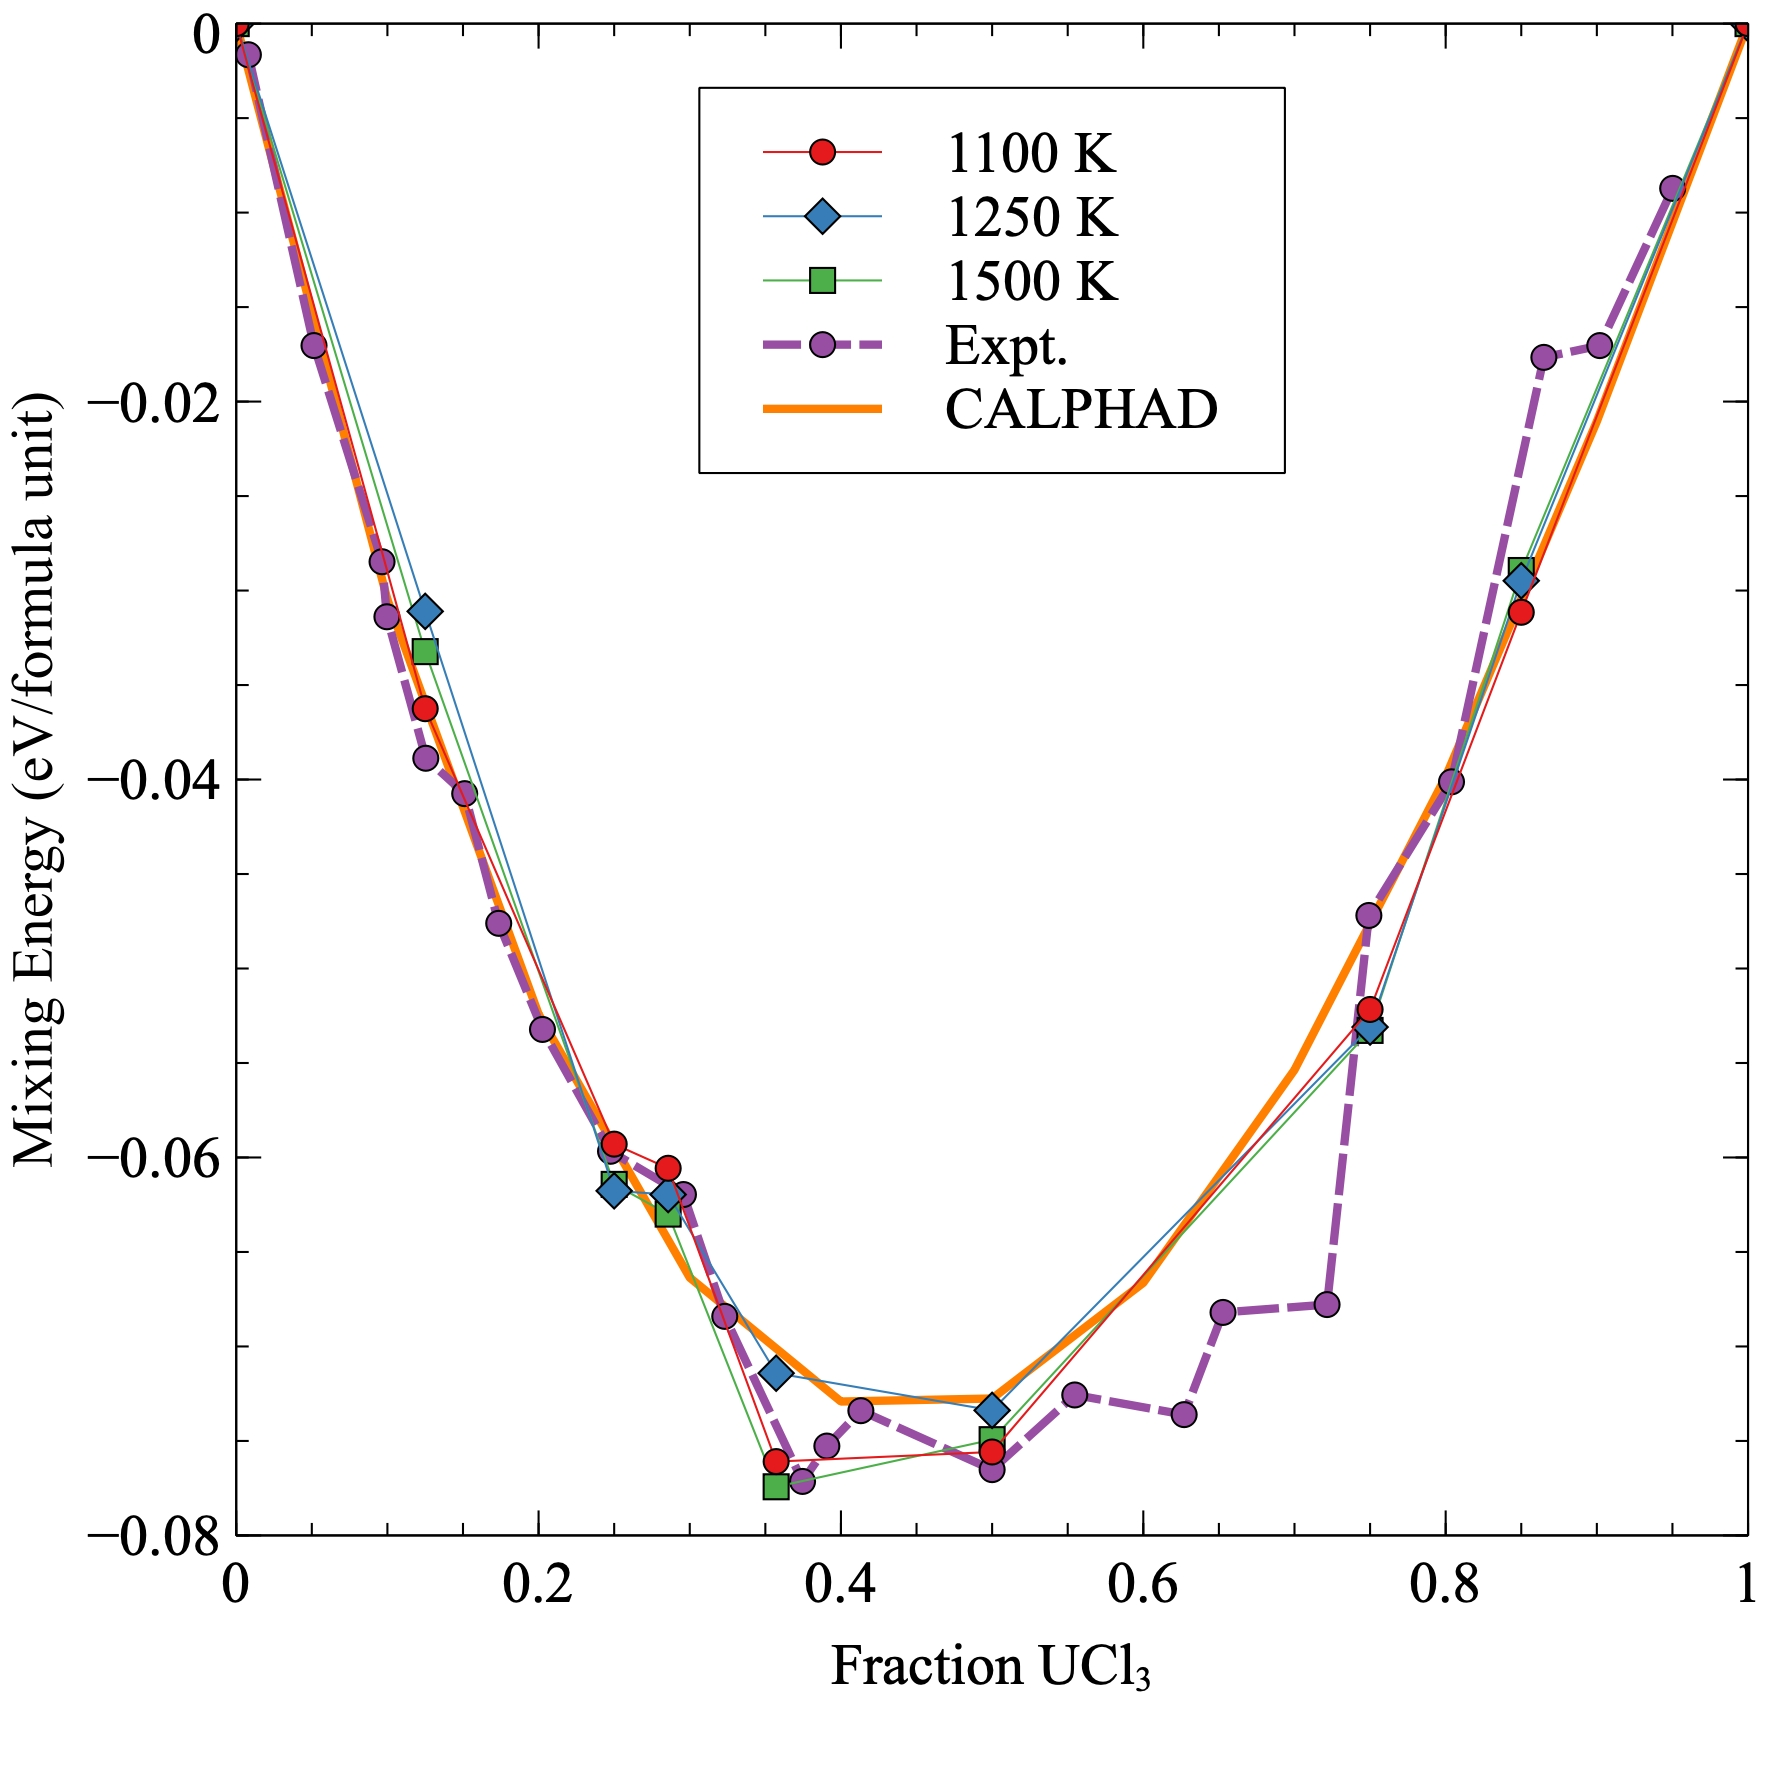
\includegraphics[width=0.5\textwidth]{fig10.jpg}
\caption{Mixing energies for NaCl-UCl$_3$ at 1100, 1250 and 1500 K. Pure NaCl and UCl$_3$ are used as references. The calculated results are compared to experiments~\cite{Matsuura} and a thermodynamic assessment~\cite{YIN2020}.%The solid black line represents the zero-mixing energy for the ideal solution. %b) Same as a) but performed using a different simulation methodology at 1200 K. 
} 
\label{fig:mixing}
\end{figure*}

Based on the results for the mixing energy, the following expression may be fitted to the mixing energy as function of the composition and temperature:
\begin{equation}
\begin{split}
E_{mix}(x,T)=(e_1+e_2T)+(f_1+f_2T)x+(g_1+g_2T)x^2+(h_1+h_2T)x^3+(i_1+i_2T)x^4\\
%+(j_1+j_2T)x^5,
\label{eq:LSE}
\end{split}
\end{equation}
where all the temperature dependent parameters are set to zero based on the lack of discernible temperature dependence in Fig. \ref{fig:mixing}. This expression is equivalent to the Redlich-Kister expansion used in existing Calphad models. The coefficients resulting from the fit to the data in Fig. \ref{fig:mixing} are summarized in Table \ref{table:LS}. heat capacity may be derived as the derivative of Eq. \ref{eq:LSE}.
%The comparison between large and small supercells for the density and mixing energy are also shown in Figs. \ref{fig:NaClUCl3} and \ref{fig:NaClUCl3e}. Unlike the cases of NaCl and UCl$_3$, the NaCl-UCl$_3$ mixture exhibit some deviation between the supercells for one of the compositions, although the trends are still the same. 

\FloatBarrier

\subsubsection{Compressibility}

The degree of compressibility of a fluid has strong implications for its dynamics. The compressibility is determined as the negative of the derivate of the volume as a function of pressure, divided by the volume at a given pressure, as in equation \ref{eq:compress}. The pressure at a series of volumes was identified and a second order polynomial was fit to the dependence. This second order polynomial served as the base function to obtain the derivative of the volume with respect to pressure. The volume of interest is identified as that at which the pressure is zero for a given temperature and composition. The temperature and composition dependent compressibility is displayed in Fig. \ref{fig:compress}. Given the isothermal nature of the simulations, this data can be considered to be isothermal compressibility. There is a decrease in the compressibility both with increasing UCl$_3$ fraction and with decreasing temperature. The magnitudes indicate a liquid that is more compressible than water at room temperature and atmospheric pressure (46$\times$10$^{-11}$ Pa$^{-1}$), less compressible than mercury (3.7 $\times$10$^{-11}$ Pa$^{-1}$), and comparable to glycerin (21$\times$10$^{-11}$ Pa$^{-1}$) \cite{aiphandbook}. As can be observed in equation \ref{eq:compress}, the compressibility is the reciprocal of the bulk modulus, and can thus be interpreted in the inverse manner. As such, UCl$_3$ has a higher bulk modulus than NaCl. Additionally, the bulk modulus softens with increasing temperature, as would be expected.  

\begin{figure}[htb]
\centering
\includegraphics[width=0.5\textwidth]{figbulk.jpg}
\caption{Calculated compressibilities for the NaCl-UCl{$_3$} pseudo-binary as a function of composition at four temperatures. Linear fits to the data are included to better illustrate trends in the data and do not imply a linear relationship.} 
\label{fig:compress}
\end{figure}

\FloatBarrier

\subsubsection{Diffusivity}
%As for NaCl, The AIMD simulations also allow calculation of the diffusivity of each species. Again similar to the NaCl system, these simulations work best in the NVT ensemble and results are only report for that case, see Fig. \ref{fig:diffUCl}. As expected, the diffusivity is a linear function of temperature. %, with a much stronger temperature dependence for Cl than for U. 
%The mobility of each species may be derived from the slope of the diffusivity as function of temperature (see Table \ref{table:NaCldiffusivityetc}). 

The diffusion coefficients for each individual species, as well as the total diffusion coefficient, are plotted as a function of composition and temperature in Fig. \ref{fig:diff}. The diffusion coefficients follow a similar trend for all compositions in temperatures in that D$_{Na}$ $>$ D$_{Cl}$ $>$ D$_U$. Additionally, the diffusion coefficients decrease with increasing UCl$_3$ content. However, the most rapid diffusion is found for the pure UCl$_3$ system. Arrhenius fits to the data can be applied, as in Fig \ref{fig:arrhenius}, and tabulated in Table \ref{tab:diff}. The migration energies as calculated from the Arrhenius fits show a near monotonic increase with increasing UCl$_3$ content. The increase in the diffusion coefficient for pure UCl$_3$ is due to the larger pre-factor. The results for NaCl compare favorably with previous experimental measurements of diffusivities. While this work predicts a Na diffusion coefficient in NaCl of 4.7$\times$10$^{-9}$ m$^2$/s, experimental measurements have determined a value of 8.0 $\times$10$^{-9}$ m$^2$/s \cite{janz_diffusion}. Additionally, Na diffusion proceeding more rapidly in NaCl than Cl diffusion has been observed experimentally \cite{janz_diffusion}. No experimental diffusion data has been obtained for the pure UCl$_3$ or the NaCl-UCl$_3$ system. 

\begin{figure}[htb]
\centering
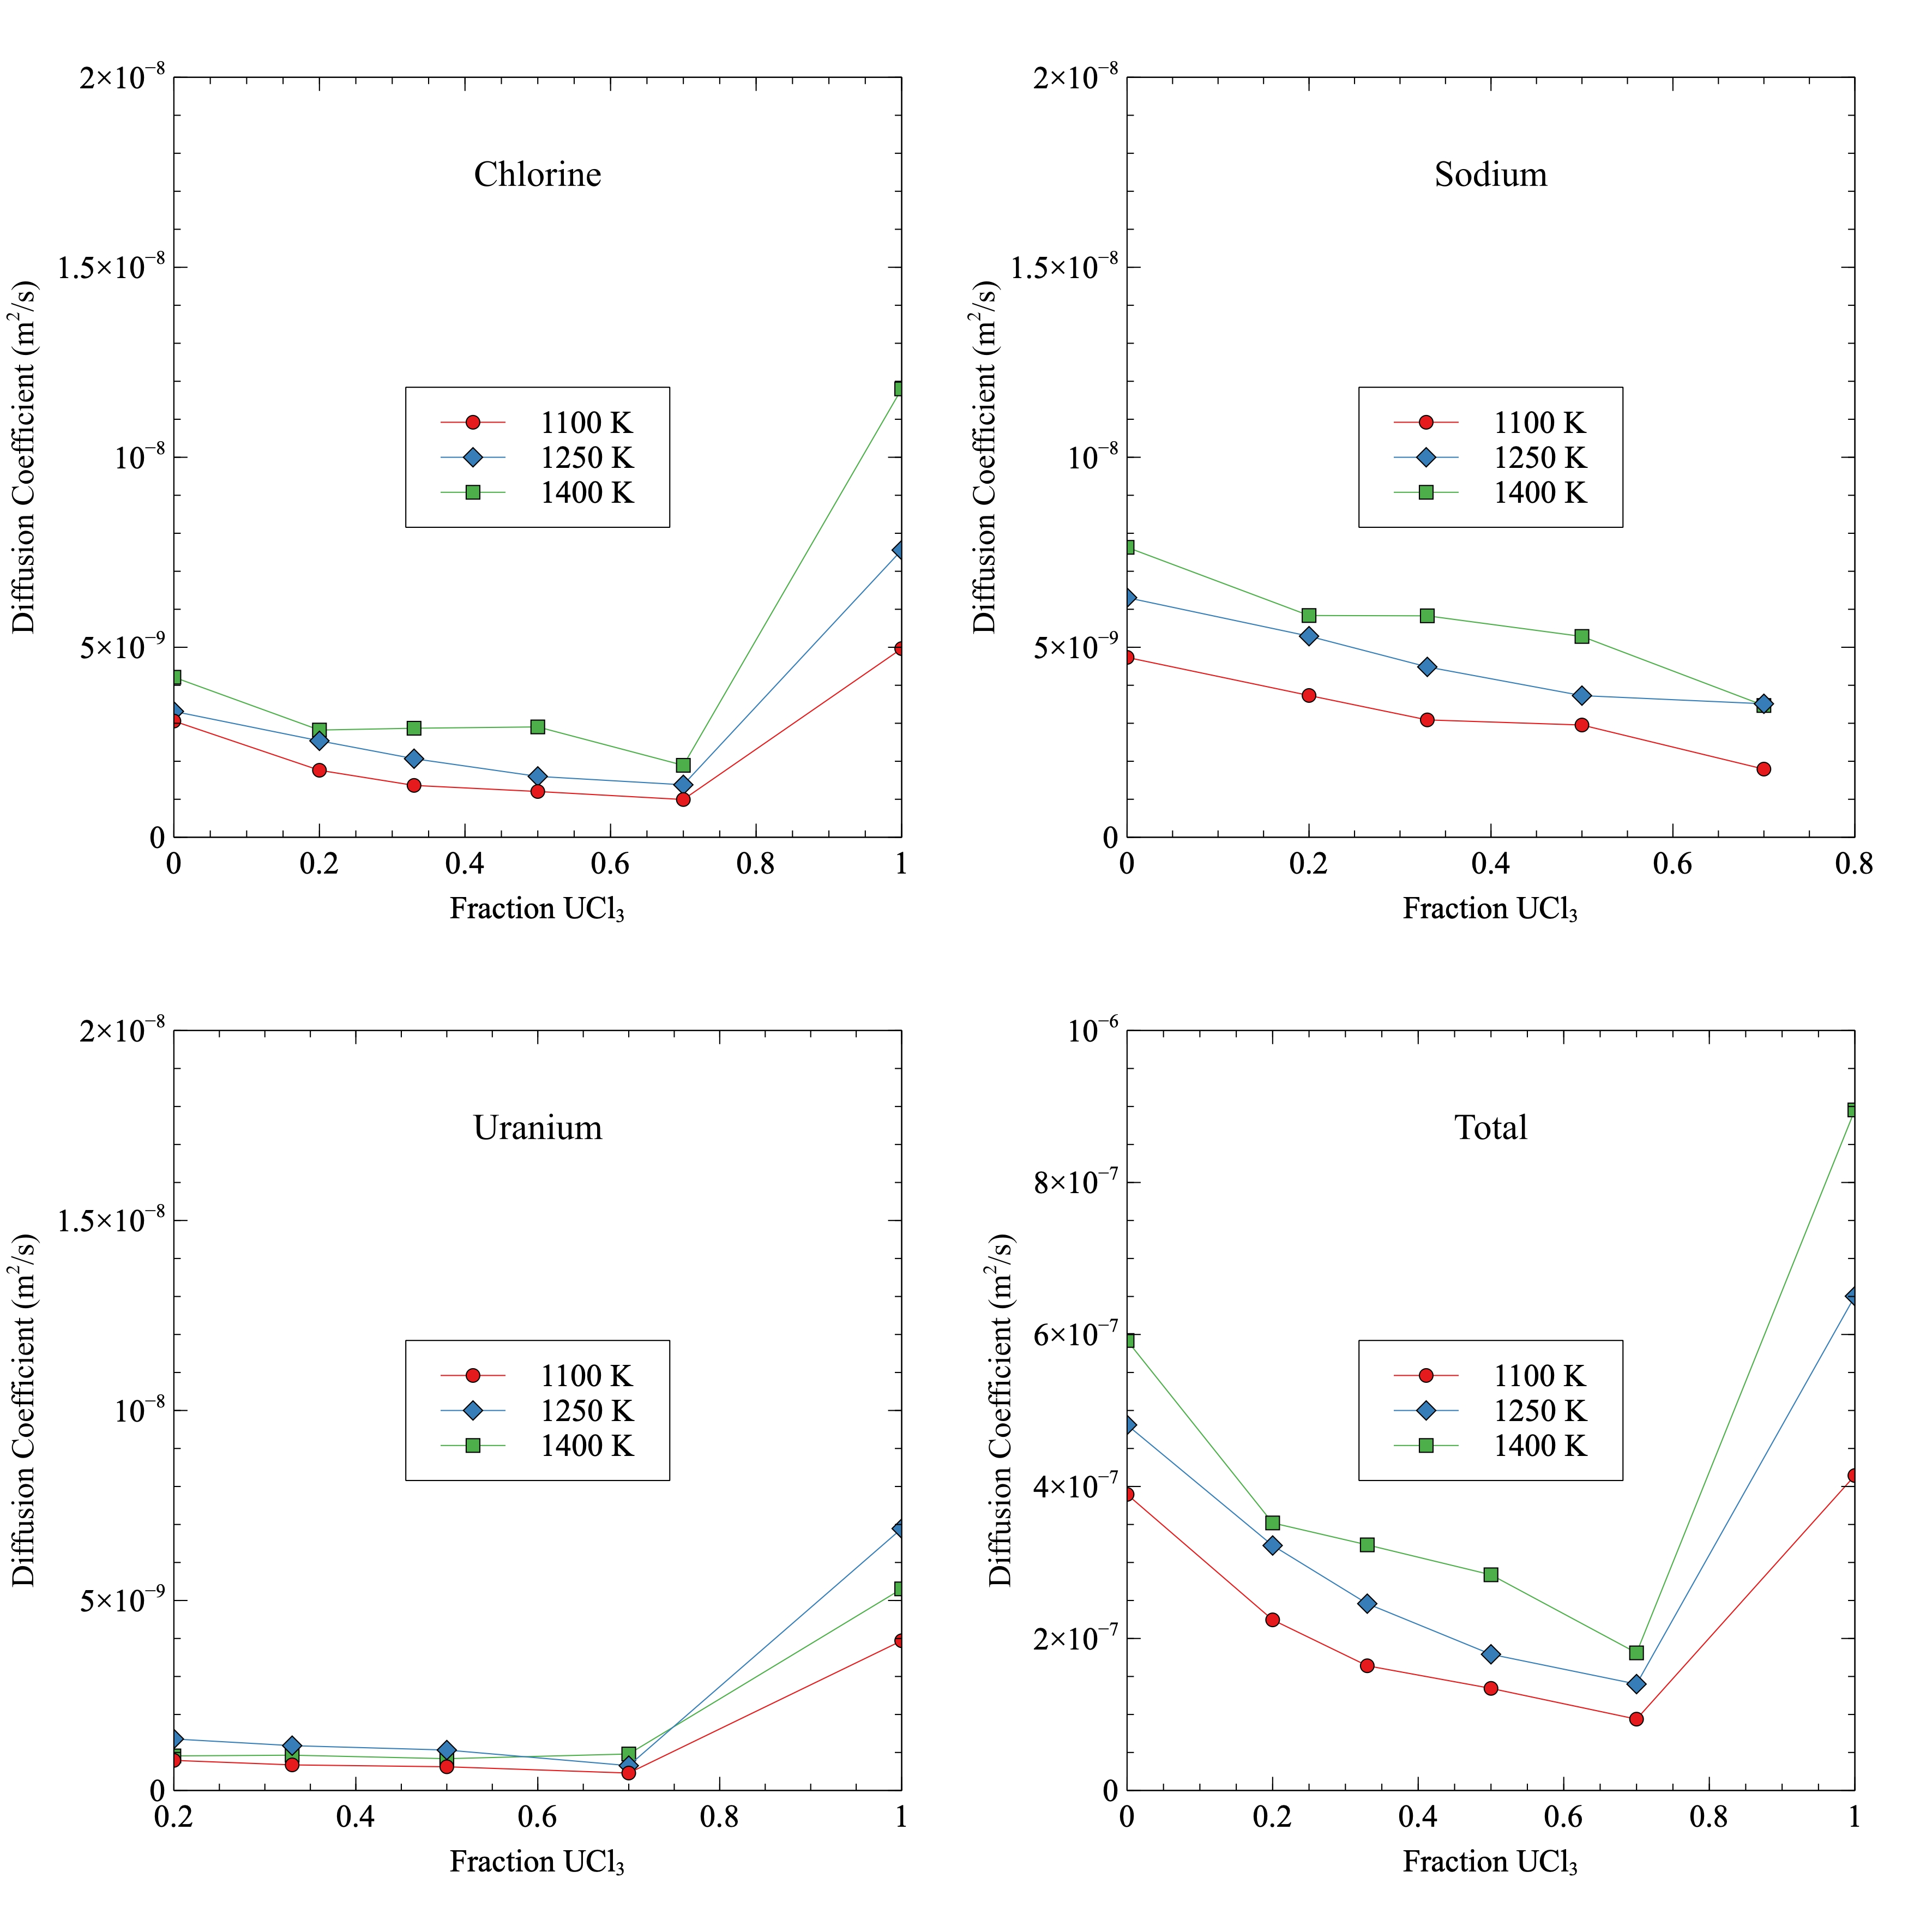
\includegraphics[width=0.9\textwidth]{diff1.jpg}
\caption{Calculated diffusivities for each species in NaCl-UCl{$_3$} and the total diffusivity as function of temperature.} 
\label{fig:diff}
\end{figure}

\begin{figure}[htb]
\centering
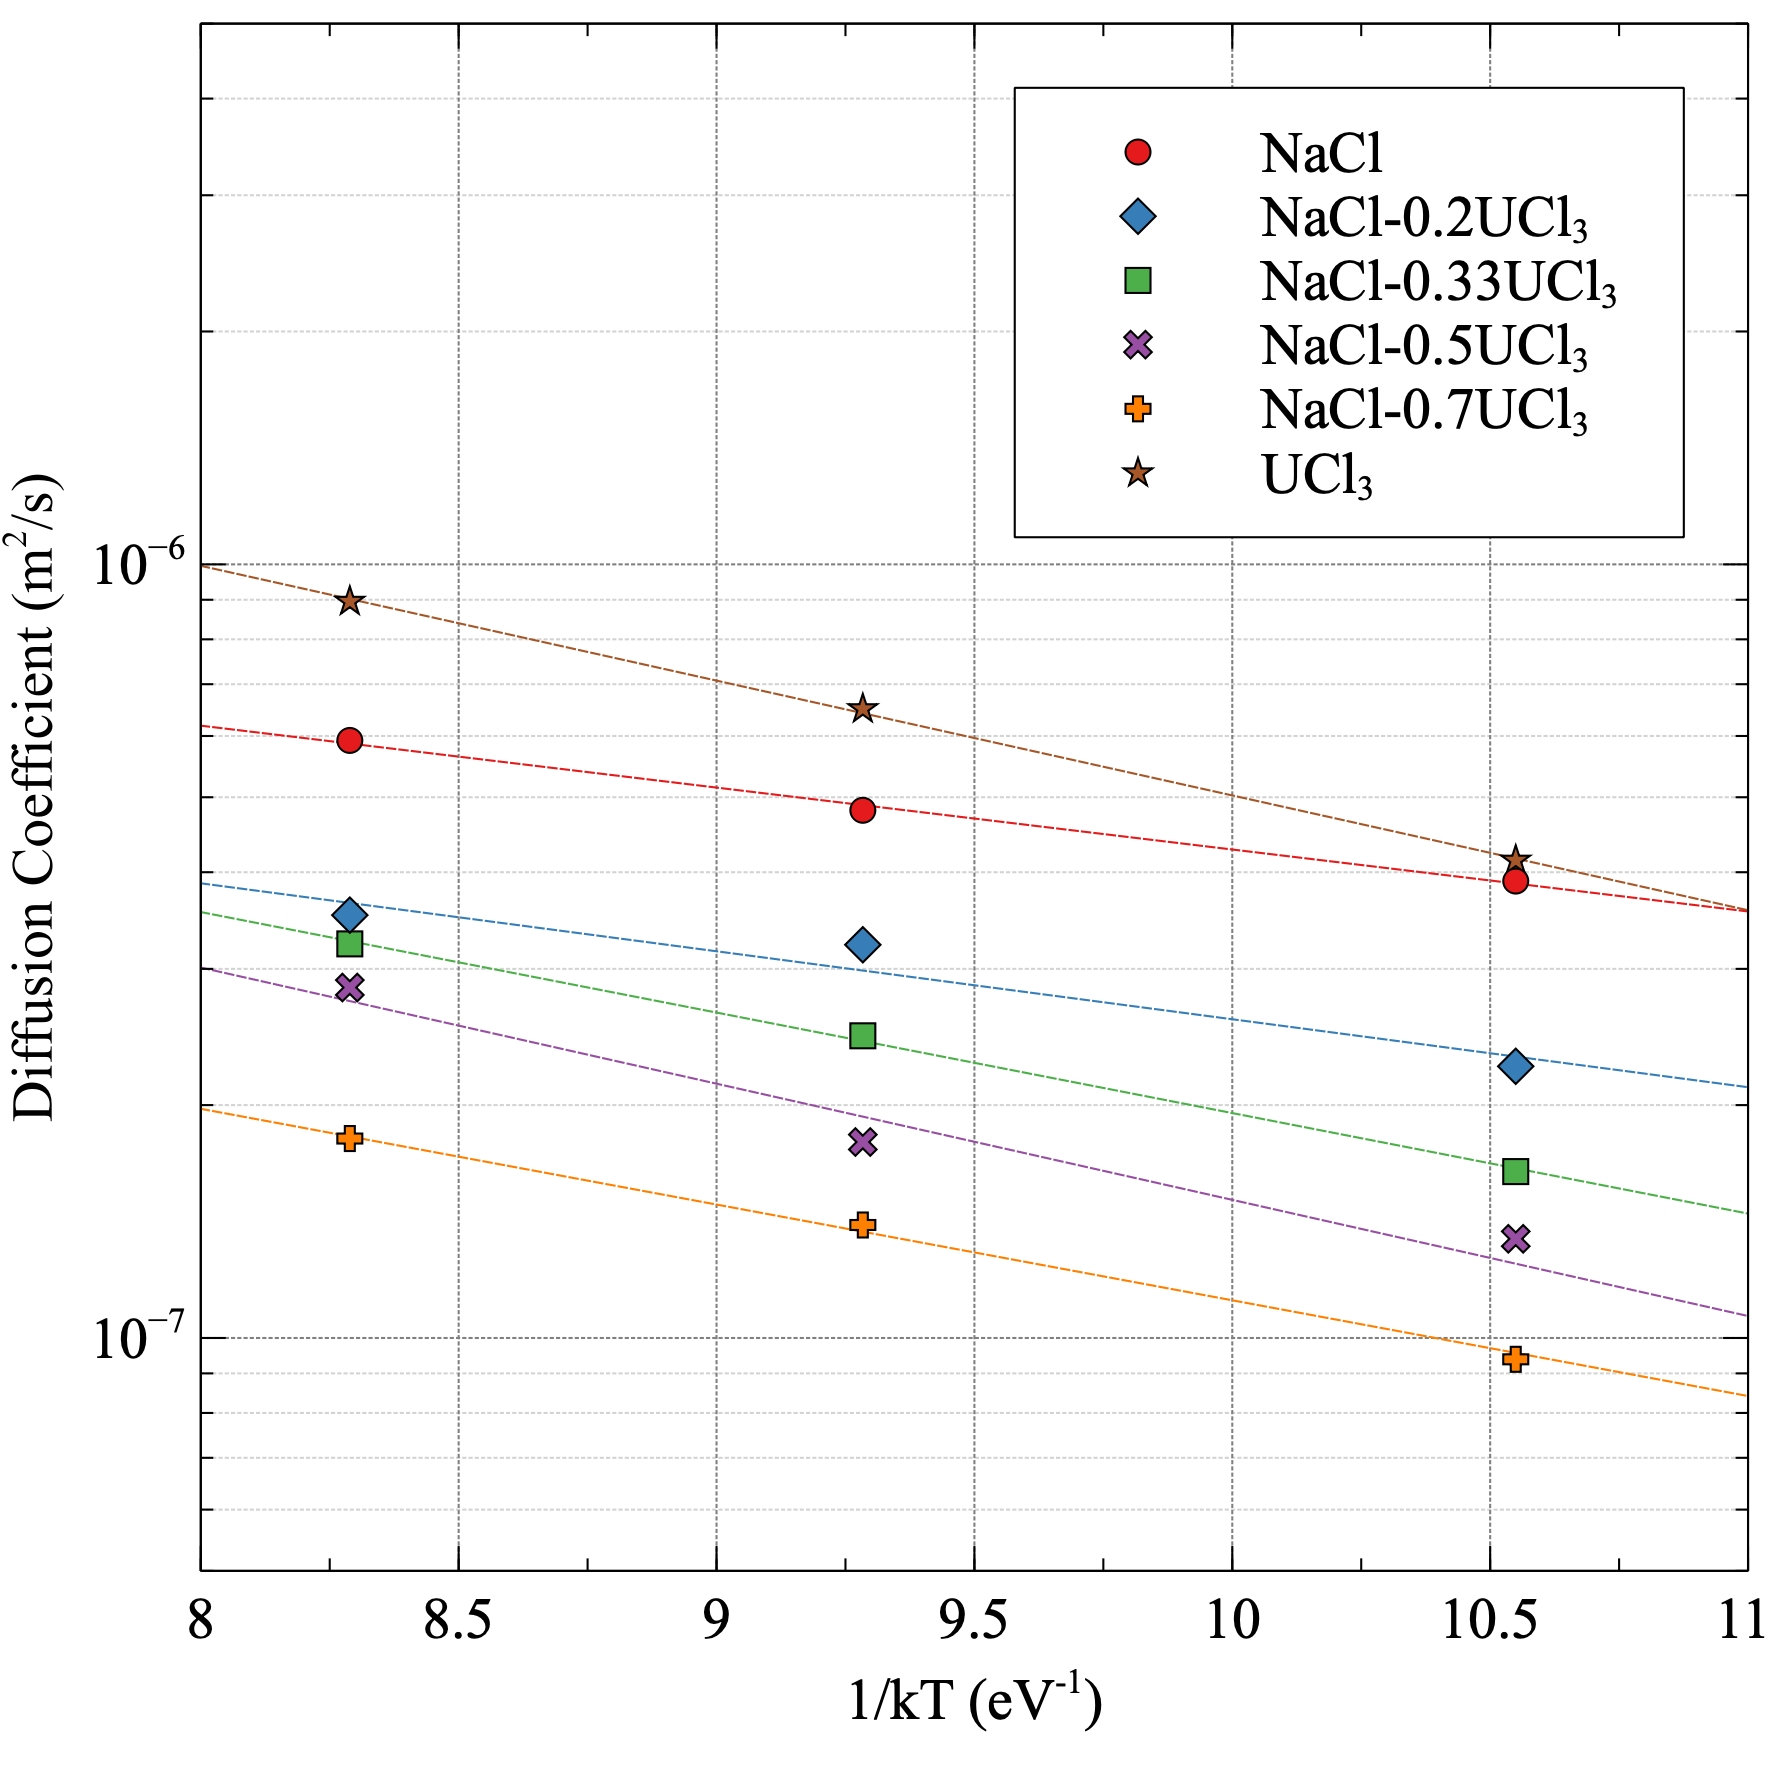
\includegraphics[width=0.5\textwidth]{arrhenius.jpg}
\caption{Arrhenius diffusion of NaCl-UCl{$_3}} 
\label{fig:arrhenius}
\end{figure}

\begin{table*}[hb!]
\centering
\caption{Prefactor and migration energy for the total diffusion of NaCl-UCl$_3$ systems.}
\begin{tabular}{lccc|}
\hline
\hline
Fraction UCl$_3$	&	D$_0$(m$^2$/s)	&	E$_m$(eV)	\\
\hline
0	&	5.41E-08	&	-0.184	\\
0.2	&	4.93E-08	&	-0.203	\\
0.33	&	1.10E-08	&	-0.301	\\
0.5	&	1.26E-07	&	-0.326	\\
0.7	&	7.10E-08	&	-0.292	\\
1	&	9.65E-07	&	-0.388	\\
\hline
\hline
\end{tabular}
\label{table:LS}
\end{table*}


\FloatBarrier

\section{Discussion}
\label{sec:discussion}
This discussion section will focus on the behavior of mixed salts, in particular how the mixing properties (energy and density) relate to the evolution of the pair distribution functions in the mixed salts. Figure \ref{fig:fig_pair} plots the pair distribution functions at four salt compositions ($x=0.25$, $x=0.29$, $x=0.36$ and $x=0.50$) and compares them to the reference pair distribution functions for UCl$_3$. 
Ref.~\cite{Li} already showed that as NaCl is added to pure UCl$_3$, the number of Cl ions in the first neighbor shell around U ions increases, from 6 in UCl$_3$ to almost 8 close to NaCl, with a corresponding decrease around Na ions. This is also confirmed in the present study (see the increase of the first peak in Figure \ref{fig:fig_pair} as the NaCl fraction increases). This redistribution of Cl ions clearly represents a favorable interaction as the mixing energy is negative across the full composition range. The same study also identified networks of UCl$_3$ units above a fractional UCl$_3$ concentration of 0.30, and more isolated units below this concentration. This behavior is also visible in the pair distribution functions. The U-U pair distribution function for mixtures with a composition equal to or above a fractional UCl$_3$ concentration of 0.36 maintain the same shape and height as in pure UCl$_3$ (they essentially overlap), which emphasizes the importance of network formation in the mixtures. 
Below a fractional concentration of 0.36 the U-U pair distribution function rapidly deviates from the pure UCl$_3$, indicating an inability to maintain the favorable network structure. This behavior is visible in the third coordination shell in Figure \ref{fig:fig_pair}.
Related changes may be observed in other distribution functions. 
The location of this transition coincides with the minimum in the mixing energy and the maximum deviation of the density from an ideal solution (compare Figures \ref{fig:fig_pair}, \ref{fig:NaClUCl3} and \ref{fig:NaClUCl3e}). In turn, these coincide with the eutectic composition according to the experimental phase diagram~\cite{YIN2020}. Combined with the evolution of the U-Cl and U-U pair distribution functions in the mixtures, this suggests that the negative mixing energy is driven by increases in the Cl coordination around U ions, but if the fractional UCl$_3$ concentration is below $\approx 0.36$, the gain from increasing this U-Cl coordination is countered by not being able to maintain the favorable U-U coordination seen in UCl$_3$, as evidenced by the break-up of the network structure. The balance of the increase in the U-Cl coordination and decrease in U-U coordination as function of the composition of NaCl-UCl$_3$ salts is responsible for the minimum in the mixing energy and by extension the location of the eutectic point in the phase diagram. 

The negative deviation from an ideal solution exhibited by the density implies that the volume increases. Often, a negative mixing energy is associated with a stronger bonding and lower volume, clearly that is opposite to what is observed for NaCl-UCl$_3$. The reason for increased volume and decreased density is again related to the evolution of the pair distribution function. The increased coordination number of Cl around U ions means that the bonding environment starts to resemble that of U$^{4+}$ ions in UCl$_4$, which may also be what drives the favorable interaction. The density of UCl$_4$ is noticeably lower (and the molar volume higher) than that of UCl$_3$, which we believe correlates with the negative deviation form an ideal mixture for the density of NaCl-UCl$_3$ mixtures. Note that this analogy does not imply  presence of formal U$^4+$ ions in NaCl-UCl$_3$, but a partial transition that drives the evolution of both the mixing energy and density. Additional simulations and experiments would be required to prove this hypothesis. What we can say is that the higher U$^{3+}$-Cl$^{-}$ coordination in the mixed salts leads to an increase in volume and a corresponding decrease in the density.

 \begin{figure*}[htb]
\centering
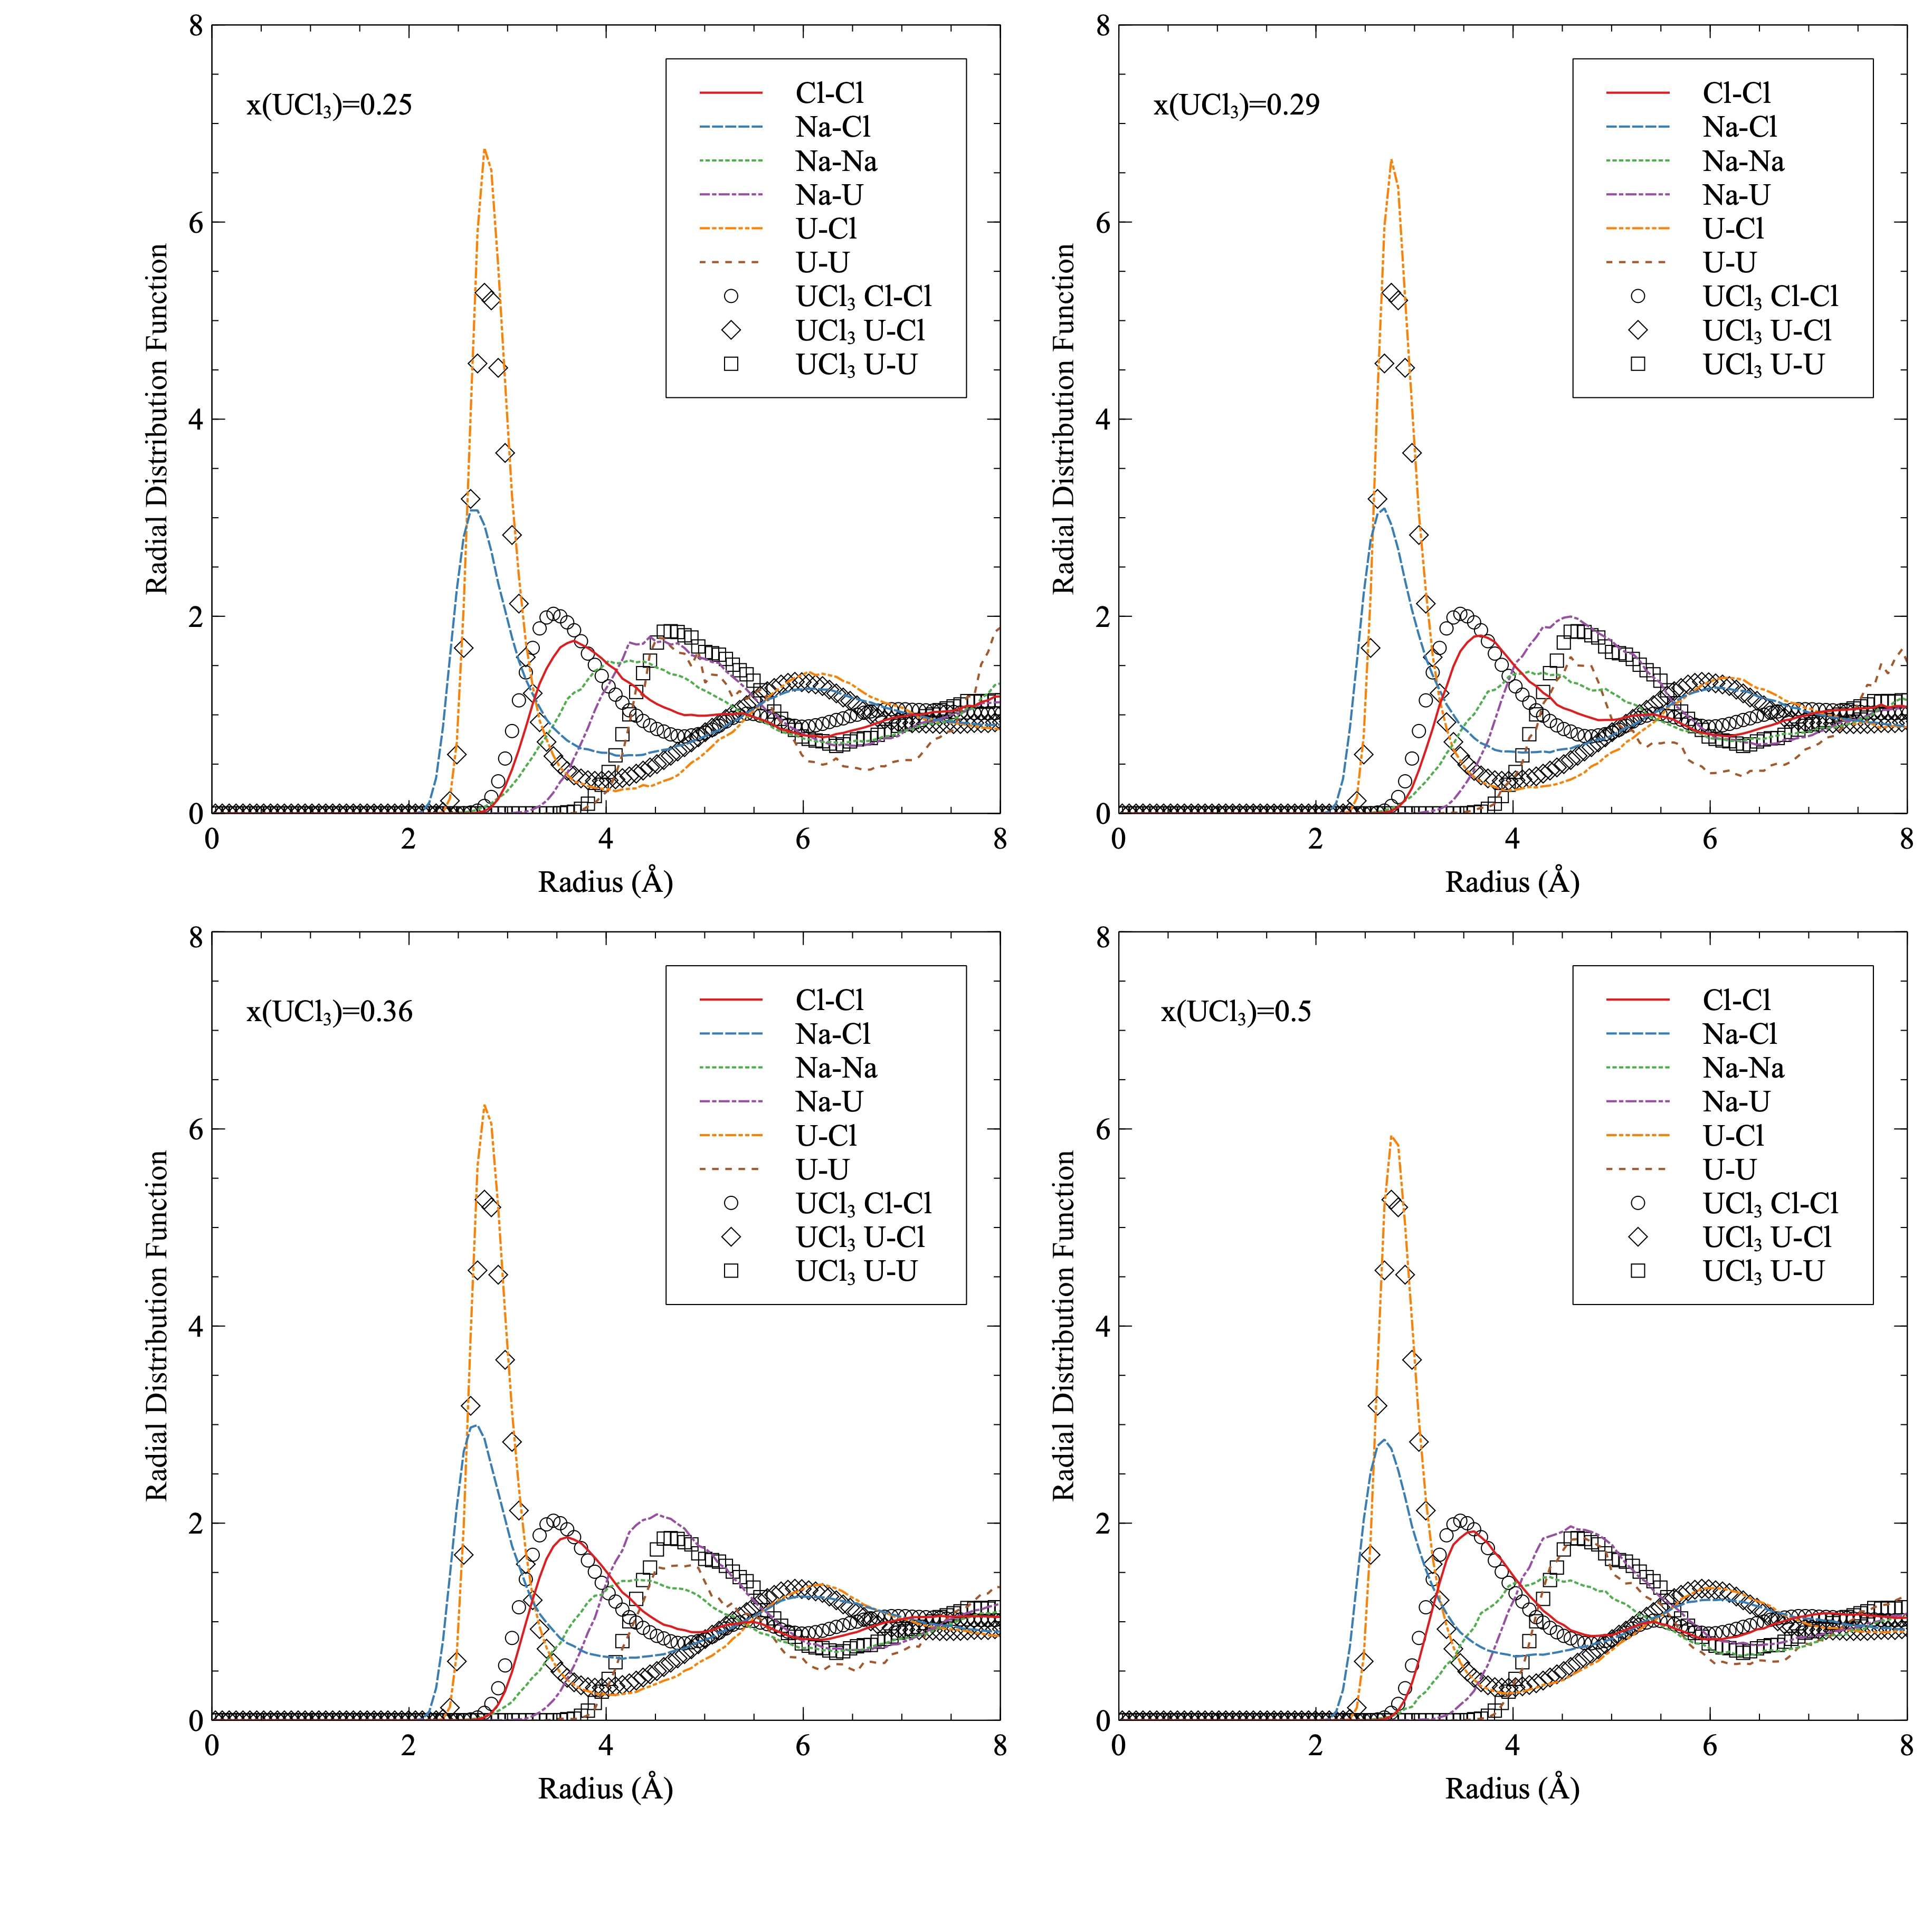
\includegraphics[width=0.95\textwidth]{fig14.jpg}
\caption{Pair distribution functions for NaCl-UCl$_3$ mixtures as function of composition ($x=0.25$, $x=0.29$, $x=0.36$ and $x=0.50$). The reference U-Cl and U-U pair distribution functions for UCl$_3$ are plotted in each figure for comparison.} 
\label{fig:fig_pair}
\end{figure*}

\FloatBarrier

\section{Summary and conclusions}
\label{sec:conclusions}
Development of next-generation molten salt reactors (MSRs) require accurate thermodynamic and thermophysical properties of fuel-bearing salt mixtures and how those change with composition as well as with addition of corrosion and fission products. The challenges associated with handling radioactive and corrosive salts make experimental measurements challenging. Using atomic scale simulations to fill these data gaps and to provide mechanistic understanding of property relations would facilitate more accurate evaluation of various concepts by reactor designers, developers and other interested parties. Modeling and simulations have an important role to play in reducing data gaps, because the compositional space of interest is extensive and difficult to cover with experiments alone, especially since some of the salts are also highly toxic or radioactive. 

Following this recipe, AIMD simulations relying on different models for Van der Waals interactions were used to predict temperature dependent thermophysical (density and thermal expansion) and thermodynamic (mixing energy and heat capacity) properties of NaCl mixed with UCl$_3$. {\color{red} Further details to be added.}
AIMD simulations of the pure end-member systems are able to accurately reproduce experimental data on densities and heat capacities provided that Van der Wals interactions are included in the simulations. The best agreement is obtained for the dDsC correlation. {\color{red} Further details to be added.} Mixtures of UCl$_3$ with NaCl exhibit a negative mixing energy, with a minimum close to the eutectic composition of $x=0.35$. For NaCl-UCl$_3$ the mixing energy is predicted to be independent of temperature. The predicted mixing energy for NaCl-UCl$_3$ agree very well with available experimental data. 
The existence of a minimum for mixing energy is related to the evolution of the radial distribution function. Addition of NaCl to UCl$_3$ increases the U-Cl coordination, which is a favorable reaction. Up until $x=0.35$ the system is able to increase this coordination number, while maintaining the intermediate range U-U correlation. This behavior is a consequence of the tendency of UCl$_3$ to form network structures. For a UCl$_3$ fraction less than approximately 0.35, the U-U coordination starts to decrease and deviate from pure UCl$_3$, which leads to a lower mixing energy (less favorable). The $x=0.35$ composition coincides with the observed eutectic composition. 
The same interactions that control the mixing energy also govern the evolution of the density for mixed salts. NaCl-UCl$_3$ exhibits a maximum deviation from ideal solution behavior at $x=0.35$. The densities of the mixed salts are lower than for the ideal mixture. The maximum deviation is about 2\% for NaCl-UCl$_3$ and 3\% for KCl-UCl$_3$. The maximum deviation is only weakly dependent on temperature, but the deviation from ideal solution behavior exhibits some temperature dependence in the UCl$_3$ rich range. The predicted densities for the mixed systems agree at least qualitatively with available experimental data. New experiments would be required to assess the quantitive accuracy of the simulations. 

\section*{Acknowledgements}
This work was funded by the U.S. Department of Energy (DOE), Office of Nuclear Energy, Nuclear Energy Advanced Modeling and Simulation (NEAMS) program. Los Alamos National Laboratory, an affirmative action/equal opportunity employer, is operated by Triad National Security LLC, for the National Nuclear Security Administration of the U.S.\ Department of Energy under Contract No. 89233218CNA000001. Los Alamos Laboratory Directed Research and Development (LDRD) is acknowledged for supporting method development and establishing simulations procedures used in part of this study.

\section*{References}

\bibliographystyle{elsarticle-num}         
\bibliography{Yellowjacket.bib}

\end{document}

